\documentclass[aps,pre,reprint,superscriptaddress,amsmath,amssymb,floatfix]{revtex4-2}

\usepackage{graphicx}
\usepackage{dcolumn}
\usepackage{bm}
\usepackage{booktabs}
\usepackage{microtype}
\usepackage{placeins}
\usepackage[colorlinks=true,linkcolor=blue,citecolor=blue,urlcolor=blue]{hyperref}

\graphicspath{{./}{figures/}{../figures/}}

\begin{document}

\title{Lattice Topology, Vacancy Clustering, and Transport: A Thermodynamic-to-Geometric Crossover in SC, BCC, and FCC Lattices}

\author{Salin Adhikari}
\email{asalinadhikari@gmail.com}
\affiliation{Rato Bangala School, Lalitpur, Nepal}

\author{Nilaksh Khetan}
\email{nilakshkhetan@gmail.com}
\affiliation{Rato Bangala School, Lalitpur, Nepal}

\date{\today}

\begin{abstract}
Vacancy-mediated diffusion scales linearly with vacancy concentration in dilute crystals ($D \propto C_v$), but attractive interactions disrupt this scaling via clustering and phase separation. To clarify how thermodynamic demixing, lattice connectivity, and conserved coarsening jointly govern vacancy organization and transport, we compare SC ($Z=6$), BCC ($Z=8$), and FCC ($Z=12$) lattices under a common attractive lattice-gas Hamiltonian and conserved Kawasaki Metropolis dynamics ($1{,}740$ unique interacting trajectories including $465$ canonical $L=20$ runs, $n=50$/point percolation crossovers, dilute $T=100$ benchmarks, and $L=40$ coarsening kinetics, plus $8{,}200$ non-interacting $J=0$ controls). All lattices recover the analytical dilute-limit prediction for $D/C_v$, $D_{\mathrm{ref}} = \frac{1}{3}f_0 r_{\mathrm{nn}}^2$, within $+0.4\%$--$+0.8\%$ at $C_v=0.015$ ($+1.1\%$--$+1.9\%$ at $C_v=0.030$). At matched subcritical $T/T_c \simeq 0.82$ ($6{,}000$ sweeps), attractive interactions shift finite-time spanning crossovers below random percolation in SC ($0.689\,p_c^{\mathrm{SC}}$, $95\%$ CI $[0.674,0.708]$) and more modestly in BCC ($0.886\,p_c^{\mathrm{BCC}}$, $95\%$ CI $[0.861,0.907]$), whereas compact droplets delay subcritical FCC slightly above its random reference ($1.044\,p_c^{\mathrm{FCC}}$, $[1.024,1.065]$). Above $T_c$, residual short-range correlations shift FCC spanning below $p_c^{\mathrm{FCC}}$ ($0.882\,p_c^{\mathrm{FCC}}$); at $C_v=0.20$, FCC expands from $f_{\max}=33.3\%$ ($P_{\mathrm{span}}=0.480$) at $J=0$ to $73.9\%$ ($P_{\mathrm{span}}=1.00$) at $J=1$, demonstrating joint geometric and interaction control. Between $L=20$ and $L=40$, subcritical FCC $f_{\max}$ drops ($61.8\% \to 38.7\%$) under preasymptotic coarsening ($R_S \propto t^{0.144}$), while final local clustering and $D$ differ by less than $0.2\%$ (the production-window mean $\bar{\mathcal{C}}$ differs by $0.47\%$). Across $31$ fixed conditions, condition-fixed-effects regression shows production-window clustering $\bar{\mathcal{C}}$ explains $49.5\%$ of within-condition $\ln D$ variance ($68.0\%$ below $T_c$, wild-bootstrap $p=0.0003$), whereas $f_{\max}$ explains only $0.4\%$ of within-condition variance and is not statistically significant. With analytical normalization $D_{\mathrm{ref}}$, an empirically fitted scaling law $D/D_{\mathrm{ref}} = 0.1189\,(C_v/p_c)^{0.628}(T/T_c)^{1.075}$ gives $R^2_{\log}=0.9407$ (LOCO-CV $0.9252$, Leave-One-Lattice-Out $0.9297$, allowing lattice-specific fit parameters increases $R^2_{\log}$ by $0.43$ percentage points).
\end{abstract}

\maketitle

\section{Introduction}
\label{sec:intro}

Point defects govern mass transport, phase stability, radiation-damage evolution, and high-temperature creep in crystalline solids~\cite{Flynn1972,Manning1968,Allnatt1993}. Lattice vacancies play a central role because atomic self-diffusion proceeds primarily through nearest-neighbor atom--vacancy exchanges. In the dilute limit ($C_v \ll 1$), classical kinetic theory developed by Bardeen and Herring~\cite{Bardeen1952}, Compaan and Haven~\cite{Compaan1956}, and Manning~\cite{Manning1968} establishes an exact proportionality between the tracer diffusivity $D$ and the vacancy fraction $C_v$, moderated by a geometric tracer correlation factor $f_0$ that captures enhanced immediate return jumps into the site just vacated. Under thermal activation, this dilute transport obeys the familiar Arrhenius law,
\begin{equation}
  D = D_A \exp\!\left(-\frac{Q}{k_B T}\right),
  \label{eq:arrhenius}
\end{equation}
where $D_A$ is the Arrhenius prefactor and $Q$ is an effective activation energy.

At elevated defect concentrations---encountered in irradiated alloys, quenched supersaturated crystals, non-stoichiometric oxides, and concentrated lattice gases---vacancies no longer act as independent carriers~\cite{Murch1977,Kehr1984,Kehr1989,Allnatt1993}. Effective attractive vacancy--vacancy interactions (equivalent to cohesive atom--atom bonding in a binary lattice gas~\cite{Lee1952,Yeomans1992}) produce short-range clustering above the demixing transition and macroscopic phase separation inside the miscibility gap. Early Monte Carlo studies of interacting lattice gases demonstrated that local ordering and short-range attraction strongly renormalize both jump frequencies and tracer correlation factors~\cite{Murch1977,Kehr1984,Kehr1989}. Crucially, crystal topology enters through two opposing physical scales as coordination number $Z$ increases from simple cubic (SC, $Z=6$) through body-centered cubic (BCC, $Z=8$) to face-centered cubic (FCC, $Z=12$): the Ising critical temperature $T_c(Z)$ rises monotonically with $Z$~\cite{Ferrenberg2018,Lundow2009}, whereas the random site-percolation threshold $p_c(Z)$ falls monotonically~\cite{Stauffer1994,Lorenz1998,Wang2013}.

Although dilute tracer correlation theory~\cite{Bardeen1952,Compaan1956,Manning1968}, equilibrium Ising criticality~\cite{Lee1952,Binder2001}, three-dimensional correlated Ising/lattice-gas percolation~\cite{MullerKrumbhaar1974,Coniglio1980,Kertesz1989,DOnorioDeMeo1990,Zhu2026} (alongside two-dimensional geometric-cluster benchmarks~\cite{Fortunato2002}), and conserved domain coarsening~\cite{Lifshitz1961,Wagner1961,Huse1986,Amar1988,Bray1994,Majumder2011} are each well-developed fields, their interplay in conserved vacancy transport~\cite{Kawasaki1966,Kawasaki1972} across three-dimensional crystal topologies remains incompletely characterized. Three specific questions motivate the present study:
\begin{enumerate}
  \item When system-spanning vacancy networks form at elevated $C_v$ over finite conserved-dynamics times, where in $(T, C_v, Z)$ space is connectivity driven by thermodynamic demixing versus stabilized by lattice percolation geometry enhanced by residual short-range correlations?
  \item Controlling both across conditions and within identical fixed $(C_v, T, \text{lattice})$ conditions, does global cluster size ($f_{\max}$) or time-aligned local defect coordination ($\bar{\mathcal{C}}$) exhibit a robust conditional association with diffusivity suppression?
  \item When normalized by the zero-free-parameter analytical dilute diffusivity $D_{\mathrm{ref}}$ and the natural scales $(p_c, T_c)$, can an empirically fitted two-variable cross-lattice scaling law generalize out-of-sample across held-out conditions and a held-out member of the three studied cubic topologies, and how much lattice-specific variance remains?
\end{enumerate}

To answer these questions, we conduct a deterministic, conserved Kawasaki Monte Carlo study of SC, BCC, and FCC supercells under an identical attractive lattice-gas Hamiltonian. Combining $1{,}740$ unique interacting trajectories (spanning $465$ canonical $L=20$ runs, high-precision $n=50$/concentration spanning sweeps, $90$ high-temperature dilute benchmarks, and $10$ $L=40$ FCC runs with direct structure-factor coarsening measurements $R_S(t)$) together with $8{,}200$ non-interacting ($J=0$) random site-percolation controls, we establish a nuanced \emph{thermodynamic-to-geometric crossover}. Below $T_c$, attractive interactions advance finite-time spanning far below random percolation in SC and moderately below in BCC, whereas compact droplet aggregation slightly delays subcritical FCC spanning above $p_c^{\mathrm{FCC}}$. Above $T_c$, FCC geometry provides a highly connected framework while residual short-range attraction shifts spanning below $p_c^{\mathrm{FCC}}$ and drives $C_v = 0.20$ to a space-filling spanning network ($f_{\max} = 73.9\%$, $P_{\mathrm{span}} = 1.00$, versus $33.3\%$ and $0.480$ at $J = 0$). Furthermore, global cluster size $f_{\max}$ depends strongly on finite-time preasymptotic coarsening and shows no detectable within-condition association with diffusivity, whereas time-aligned local clustering $\bar{\mathcal{C}}$ retains a strong negative conditional association with $\ln D$ supported by exact atom--vacancy interface conservation, and an empirically fitted cross-lattice scaling law under analytical normalization $D_{\mathrm{ref}}$ retains predictive accuracy when each of the three studied cubic topologies is held out in turn.

\section{Model and Computational Methods}
\label{sec:methods}

\subsection{Lattice Geometries and Exact Ising Mapping}
\label{sec:lattice_models}

We simulate periodic SC, BCC, and FCC supercells of $L \times L \times L$ conventional cubic unit cells with lattice parameter $a = 1$. Accounting for their crystallographic bases ($1$, $2$, and $4$ sites per unit cell), the primary $L = 20$ supercells contain $N = 8{,}000$ (SC), $16{,}000$ (BCC), and $32{,}000$ (FCC) sites; finite-size $J=0$ FCC controls also probe $L = 30$ ($N = 108{,}000$) and $L = 40$ ($N = 256{,}000$), while interacting $L = 40$ FCC benchmarks contain $N = 256{,}000$ sites. In conventional cubic units ($a = 1$), the squared nearest-neighbor jump lengths are $r_{\mathrm{nn}}^2 = 1$ (SC), $3/4$ (BCC), and $1/2$ (FCC).

Each site $i \in \{1,\dots,N\}$ carries an occupation variable $n_i \in \{0,1\}$ ($n_i = 1$ for an atom, $n_i = 0$ for a vacancy) at fixed vacancy concentration $C_v = N^{-1}\sum_i (1 - n_i)$. Configurational interactions are governed by the attractive nearest-neighbor lattice-gas Hamiltonian,
\begin{equation}
  E(\{n_i\}) = -J \sum_{\langle i,j \rangle} n_i n_j,
  \label{eq:hamiltonian}
\end{equation}
summed over undirected nearest-neighbor pairs $\langle i,j\rangle$, with reduced units $J = 1$ and $k_B = 1$ (and $J = 0$ in non-interacting random-occupancy controls).

Substituting the Lee--Yang spin transformation $n_i = (1 + s_i)/2$ ($s_i \in \{-1, +1\}$)~\cite{Lee1952,Yeomans1992} maps Eq.~\eqref{eq:hamiltonian} directly onto the ferromagnetic spin-$1/2$ Ising model:
\begin{align}
  E &= -J \sum_{\langle i,j \rangle} \frac{(1 + s_i)(1 + s_j)}{4} \nonumber \\
    &= -\frac{J}{4} \sum_{\langle i,j \rangle} s_i s_j - \frac{ZJ}{4} \sum_{i=1}^N s_i - \frac{ZNJ}{8}.
  \label{eq:ising_map}
\end{align}
Because Kawasaki dynamics conserves total atom number $\sum_i n_i = N(1 - C_v)$, the total spin $\sum_i s_i = N(1 - 2C_v)$ is strictly invariant along every trajectory. The linear and constant terms in Eq.~\eqref{eq:ising_map} therefore drop out of all energy differences, establishing exact canonical equivalence to the conserved-magnetization Ising model with effective coupling
\begin{equation}
  J_{\mathrm{Ising}} = \frac{J}{4} = 0.25
  \label{eq:j_ising}
\end{equation}
and reduced magnetization $m = 1 - 2C_v$. The lattice-gas critical temperature accordingly satisfies $T_c^{\mathrm{LG}}/J = (k_B T_c^{\mathrm{Ising}}/J_{\mathrm{Ising}})/4$. Using high-precision three-dimensional Ising benchmarks---$k_B T_c^{\mathrm{Ising}}/J_{\mathrm{Ising}} = 4.511523$ (SC)~\cite{Ferrenberg2018}, $6.35435$ (BCC), and $9.7952$ (FCC)~\cite{Lundow2009}---yields
\begin{equation}
  T_c^{\mathrm{SC}} = 1.13, \qquad T_c^{\mathrm{BCC}} = 1.59, \qquad T_c^{\mathrm{FCC}} = 2.45,
  \label{eq:tc_values}
\end{equation}
matching $T_c^{\mathrm{Ising}}/4$ ($1.1279$, $1.5886$, $2.4488$) to three significant figures.

Since our concentrated production runs ($C_v \in [0.14, 0.25]$) lie off the critical composition ($m = 1 - 2C_v \in [0.50, 0.72]$), we verify their placement relative to the coexistence binodal $m_{\mathrm{coex}}(T)$. Evaluating the Talapov--Bl\"ote three-dimensional Ising magnetization formula~\cite{Talapov1996} at $T/T_c = 0.82$ gives $m_{\mathrm{coex}} \approx 0.840$, corresponding to a coexistence vacancy fraction $C_v^{\mathrm{coex}} = (1 - m_{\mathrm{coex}})/2 \approx 0.080$. The sampled concentrations at $T/T_c \simeq 0.82$ therefore lie within the estimated two-phase miscibility gap ($C_v > C_v^{\mathrm{coex}}$), whereas every run at $T/T_c \simeq 1.25$ lies strictly inside the homogeneous supercritical phase.

For geometric normalization, we use the standard three-dimensional infinite-lattice random site-percolation thresholds~\cite{Stauffer1994,Lorenz1998,Wang2013}:
\begin{equation}
  p_c^{\mathrm{SC}} = 0.3116, \qquad p_c^{\mathrm{BCC}} = 0.2455, \qquad p_c^{\mathrm{FCC}} = 0.1996.
  \label{eq:pc_values}
\end{equation}
Modern large-scale estimates ($0.311608$, $0.245962$, and $0.199235$~\cite{Lorenz1998,Wang2013}) differ from Eq.~\eqref{eq:pc_values} by $< 0.2\%$. In addition, we directly measure finite-size non-interacting ($J=0$) spanning crossovers $C_v^{*,J=0}(L)$ on our exact periodic supercells (Sec.~\ref{sec:fcc_sweep}) so that finite-size geometric shifts and interaction-induced shifts~\cite{MullerKrumbhaar1974,Coniglio1980,Kertesz1989,DOnorioDeMeo1990,Zhu2026} are separated cleanly. Table~\ref{tab:lattice_specs} collects all reference constants.

\begin{table*}[t]
\caption{\label{tab:lattice_specs}Crystallographic, thermodynamic, geometric, and transport reference constants for the three cubic lattices in conventional unit-cell coordinates ($a=1$, $L=20$, $J=1$, $k_B=1$). Here $N$ is the $L=20$ site count, $Z$ the coordination number, $r_{\mathrm{nn}}^2$ the squared nearest-neighbor jump length, $f_0$ the exact dilute Bardeen--Herring/Compaan--Haven correlation factor~\cite{Compaan1956,Manning1968}, $D_{\mathrm{ref}} = \frac{1}{3}f_0 r_{\mathrm{nn}}^2$ the zero-free-parameter analytical dilute diffusivity scale (in $a^2/\mathrm{MCS}$), $D_{\mathrm{scale}}$ the secondary empirical reference scale compared in Sec.~\ref{sec:reduced_scaling}, $T_c^{\mathrm{LG}} = T_c^{\mathrm{Ising}}/4$ the critical temperature~\cite{Ferrenberg2018,Lundow2009}, and $p_c$ the infinite-lattice random site-percolation threshold~\cite{Stauffer1994,Lorenz1998}.}
\begin{ruledtabular}
\begin{tabular}{lcccccccc}
Lattice & $N$ ($L=20$) & $Z$ & $r_{\mathrm{nn}}^2$ ($a^2$) & $f_0$ & $D_{\mathrm{ref}}$ ($a^2/\mathrm{MCS}$) & $D_{\mathrm{scale}}$ ($a^2/\mathrm{MCS}$) & $T_c^{\mathrm{LG}}$ & $p_c$ \\
\colrule
SC  & $8{,}000$  & $6$  & $1.00$ & $0.6531$ & $0.2177$ & $0.1890$ & $1.13$ & $0.3116$ \\
BCC & $16{,}000$ & $8$  & $0.75$ & $0.7272$ & $0.1818$ & $0.1488$ & $1.59$ & $0.2455$ \\
FCC & $32{,}000$ & $12$ & $0.50$ & $0.7815$ & $0.1303$ & $0.1006$ & $2.45$ & $0.1996$ \\
\end{tabular}
\end{ruledtabular}
\end{table*}

\subsection{Conserved Kawasaki Dynamics and Sample Accounting}
\label{sec:dynamics}

Time evolution proceeds via conserved nearest-neighbor Kawasaki atom--vacancy exchanges under Metropolis acceptance rules~\cite{Metropolis1953,Kawasaki1966,Kawasaki1972}. One Monte Carlo sweep (MCS) consists of $N$ attempted pair swaps: a site $i$ is selected uniformly from $\{1,\dots,N\}$ and paired with a uniformly chosen nearest neighbor $j \in \mathcal{N}(i)$. If $n_i = n_j$, the move is null. Otherwise, let $u$ be the occupied site ($n_u = 1$) and $v$ the vacant site ($n_v = 0$), with pre-swap occupied neighbor counts $m_u = \sum_{w \in \mathcal{N}(u)} n_w$ and $m_v = \sum_{w \in \mathcal{N}(v)} n_w$. Prior to exchange, atom $u$ forms $m_u$ atom--atom bonds (since $n_v = 0$); after moving to $v$, site $u$ is vacant, so the moved atom forms $m_v - 1$ bonds. The exact energy change is therefore
\begin{equation}
  \Delta E = -J\bigl[(m_v - 1) - m_u\bigr] = J(m_u - m_v + 1),
  \label{eq:delta_e}
\end{equation}
accepted with probability $W(\Delta E) = \min\!\left[1, \exp(-\Delta E / T)\right]$. Because ordered-pair selection is symmetric ($P_{\mathrm{prop}}(u \leftrightarrow v) = P_{\mathrm{prop}}(v \leftrightarrow u) = 2/(NZ)$), this rule strictly obeys detailed balance with respect to the canonical Boltzmann distribution at fixed $C_v$. Boltzmann weights $\exp(-Jk/T)$ ($k \in \{0,\dots,Z\}$) are precomputed, and each run uses a unique deterministic $64$-bit seed derived via SHA-256 hashing of the run parameters (verified distinct with zero collisions across all $1{,}740$ unique interacting trajectories) feeding a \texttt{xoshiro256**} generator. Across all $465$ canonical trajectories, acceptance rates range from $10.3\%$ to $26.1\%$, confirming sustained microscopic mobility without kinetic arrest.

Each $6{,}000$-MCS production trajectory starts from a uniformly random vacancy configuration and executes a $2{,}000$-MCS burn-in followed by a $4{,}000$-MCS production window during which both the mean-squared displacement (MSD) and the instantaneous local clustering index $\mathcal{C}(t)$ are sampled at $25$ evenly spaced checkpoints ($\Delta t \in [1, 4{,}000]$ MCS). Below $T_c$ inside the miscibility gap, conserved Kawasaki dynamics does not reach global equilibrium within $6{,}000$ MCS; instead, domains undergo slow conserved coarsening governed asymptotically by Lifshitz--Slyozov--Wagner (LSW) kinetics, $R(t) \sim t^{1/3}$~\cite{Lifshitz1961,Wagner1961,Bray1994}, with well-documented preasymptotic corrections at early-to-intermediate Monte Carlo times~\cite{Huse1986,Amar1988,Majumder2011}. Accordingly, subcritical structural metrics and spanning probabilities measured at $t = 6{,}000$ MCS represent \emph{finite-time kinetic morphology regimes} at matched sweep age---not equilibrium critical percolation thresholds---whose domain growth we track directly via time-resolved structure factors $R_S(t)$, whereas quasi-stationary diffusive transport over the production window is verified directly via MSD linearity.

To keep sample provenance transparent across overlapping analyses, Table~\ref{tab:sample_accounting} summarizes the datasets, their overlap with the canonical ensemble, and the resulting number of unique trajectories. The canonical $L=20$ ensemble contains $31$ conditions with $15$ seeds per condition, giving $465$ trajectories. The SC conditions use $C_v\in\{0.15,0.20,0.25\}$ and $T\in\{0.93,1.41,2.00\}$, corresponding to $T/T_{\mathrm{c}}=0.823$, $1.248$, and $1.770$ ($135$ trajectories). The BCC conditions use the same three vacancy concentrations and $T\in\{1.30,1.99\}$, corresponding to $T/T_{\mathrm{c}}=0.818$ and $1.252$ ($90$ trajectories). The FCC concentration sweep uses $C_v\in\{0.14,0.15,0.16,0.18,0.20,0.22,0.24,0.25\}$ at $T\in\{2.00,3.06\}$, corresponding to $T/T_{\mathrm{c}}=0.816$ and $1.249$ ($240$ trajectories).

The FCC concentration sweep ($240$ trajectories) and matched reduced-temperature controls ($120$ trajectories) are subsets of the canonical $465$ and are not counted again. The high-precision spanning sweeps comprise $25$ transition-window concentrations with $50$ seeds per concentration ($1{,}250$ trajectory records). Of these, $75$ trajectories are seed-identical to canonical runs: five overlapping conditions with $15$ seeds each (SC at $C_v=0.20$; BCC at $C_v=0.20$ and $0.25$; FCC at $T=2.00$, $C_v=0.20$; and FCC at $T=3.06$, $C_v=0.18$). The spanning sweeps therefore add $1{,}175$ new trajectories, giving $1{,}640$ unique $L=20$, $6{,}000$-MCS trajectories. Combining the $1{,}250$ transition-window records with the $255$ canonical outer-tail records ($17$ conditions with $15$ seeds each) gives the $1{,}505$-trajectory spanning dataset analyzed in Table~\ref{tab:spanning}.

The complete study contains $1{,}740$ unique interacting trajectories: the $1{,}640$ unique $L=20$ runs, $90$ dilute $T=100$ benchmarks, and $10$ additional $L=40$ FCC runs. Fifteen canonical $L=20$ trajectories and five $L=40$ trajectories were continued to $10{,}000$ MCS for the coarsening analysis; these continuations are not additional independent trajectories. The study also includes $8{,}200$ independent non-interacting ($J=0$) random-occupancy configurations. Figure~\ref{fig:snapshots} shows representative $L=20$ subcritical vacancy morphologies after $6{,}000$ MCS.

\begin{table*}[t]
\caption{\label{tab:sample_accounting}Sample-count accounting for all simulation ensembles and analysis subsets. ``Entries'' denotes trajectory rows or time-checkpoint records, as identified in the footnotes. ``Previously counted'' denotes entries already included in an earlier ensemble. The total is $1{,}740$ unique interacting trajectories, plus $8{,}200$ separate non-interacting ($J=0$) static configurations.}
\begingroup
\scriptsize
\setlength{\tabcolsep}{2pt}
\renewcommand{\arraystretch}{1.12}
\begin{ruledtabular}
\begin{tabular*}{\textwidth}{@{\extracolsep{\fill}}lcccccc}
Ensemble / dataset
& $L$
& \shortstack{Sweeps\\(MCS)}
& \shortstack{Conditions\\$\times$ seeds}
& Entries
& \shortstack{Previously\\counted}
& \shortstack{Net\\new} \\
\colrule
Dilute-limit validation ($T=100$; SC/BCC/FCC)
& 20 & 2{,}000 & $6 \times 15$ & 90 & 0 & 90 \\
Canonical production ensemble (31 conditions; 15 seeds each)
& 20 & 6{,}000 & $31 \times 15$ & 465 & 0 & 465 \\
\quad FCC concentration sweep (subset)
& 20 & 6{,}000 & $16 \times 15$ & 240 & 240 & 0 \\
\quad Matched reduced-$T$ controls (subset)
& 20 & 6{,}000 & $8 \times 15$ & 120 & 120 & 0 \\
High-precision $J=1$ crossover windows
& 20 & 6{,}000 & $25 \times 50$ & 1{,}250 & 75 & 1{,}175 \\
Merged spanning set (windows + outer tails)$^{a}$
& 20 & 6{,}000 & $25 \times 50 + 17 \times 15$ & 1{,}505 & 330 & 0 \\
Finite-size FCC benchmark ($C_v=0.20$, $T=2.00$)
& 20, 40 & 6{,}000 & $15\,(L=20)+10\,(L=40)$ & 25 & 15 & 10 \\
Coarsening checkpoint records$^{b}$
& 20, 40 & 10{,}000 & $15\,(L=20)+5\,(L=40)$ & 215 & 20 & 0 \\
\colrule
\textbf{Total unique interacting ($J=1$) trajectories}
& \textbf{20, 40} & \textbf{2{,}000--10{,}000} & --- & --- & --- & \textbf{1{,}740} \\
Non-interacting ($J=0$) random controls
& 20, 30, 40 & Static & $34 \times 200 + 14 \times 100$ & 8{,}200 & 0 & 8{,}200 \\
\end{tabular*}
\end{ruledtabular}
\vspace{3pt}
\begin{minipage}{\textwidth}
\scriptsize
$^{a}$ The merged spanning set contains the $1{,}175$ new trajectories from the crossover windows plus $330$ canonical trajectories already counted above ($75$ within the transition windows and $255$ outer-tail runs); it therefore contributes no additional unique trajectories.\\
$^{b}$ The $215$ entries are time-checkpoint records, not independent trajectories. They are generated by continuing the $15$ canonical $L=20$ runs and $5$ of the $10$ $L=40$ benchmark runs to $10{,}000$ MCS; the remaining $5$ $L=40$ runs contribute checkpoints through $6{,}000$ MCS. All $20$ trajectories were counted in the canonical or finite-size rows above.
\end{minipage}
\endgroup
\end{table*}

\begin{figure*}[t]
  \centering
  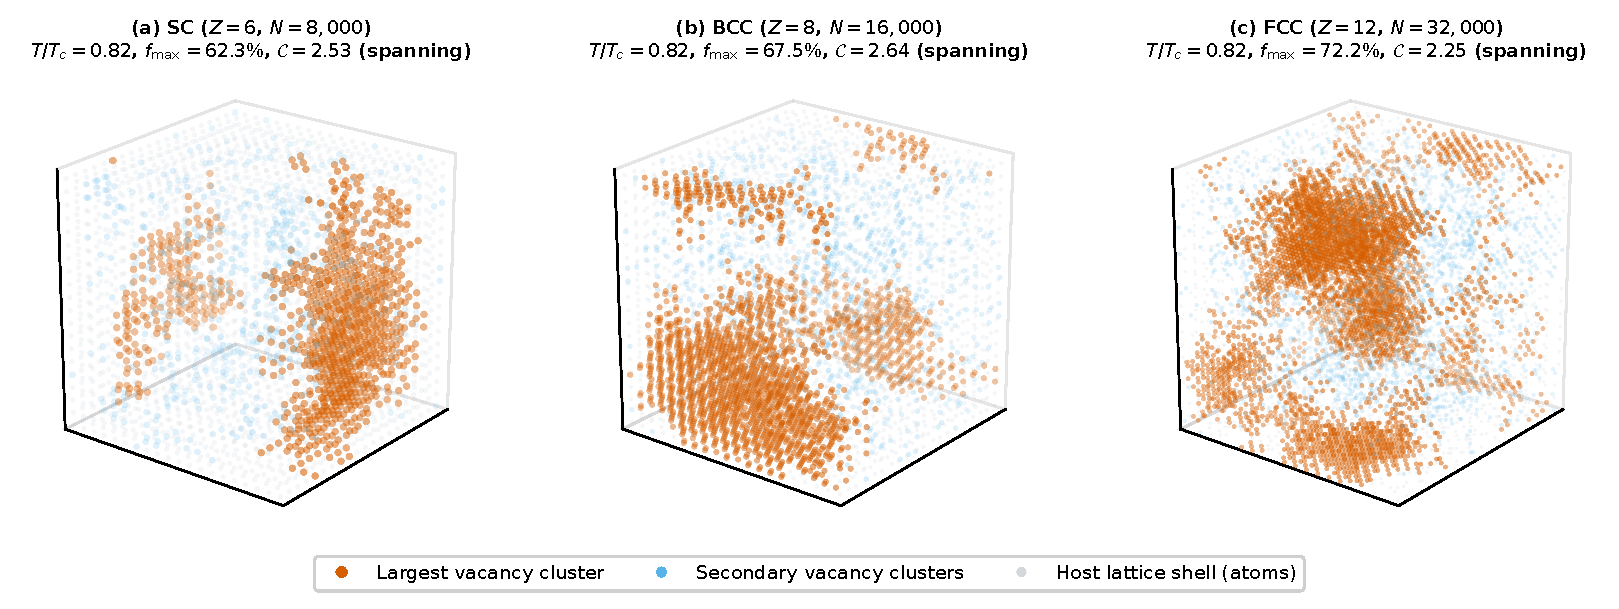
\includegraphics[width=0.98\textwidth]{fig01_vacancy_configurations.pdf}
  \caption{\label{fig:snapshots}Representative $3\mathrm{D}$ vacancy configurations at $C_v = 0.20$ and matched subcritical temperature $T/T_c \simeq 0.82$ ($L=20$, $6{,}000$ MCS, seed index $0$) for (a) SC ($T = 0.93$, $N=8{,}000$), (b) BCC ($T = 1.30$, $N=16{,}000$), and (c) FCC ($T = 2.00$, $N=32{,}000$). Vermilion spheres show the largest connected vacancy cluster, blue spheres secondary vacancy clusters, and translucent gray spheres the host-atom boundary shell. All three snapshots exhibit pronounced local clustering ($\mathcal{C} \in [2.25, 2.64]$) and compact coarsening vacancy domains.}
\end{figure*}

\subsection{Transport, Structural, and Coarsening Observables}
\label{sec:observables}

\subsubsection{Unwrapped Diffusivity and Zero-Free-Parameter Analytical Scale}

Each tagged atom $a \in \{1,\dots,N_{\mathrm{atoms}}\}$ accumulates a continuous unwrapped displacement $\mathbf{r}_a(t)$ updated by exact minimum-image jump vectors $\pm \mathbf{d}_{ij}$ upon every accepted swap, eliminating periodic boundary artifacts. Over the $4{,}000$-MCS production window (referenced to $t_0 = 2{,}000$ MCS), the ensemble-averaged MSD $\langle R^2(\Delta t) \rangle = N_{\mathrm{atoms}}^{-1}\sum_a \|\mathbf{r}_a(t_0 + \Delta t) - \mathbf{r}_a(t_0)\|^2$ is fitted by ordinary least squares (OLS) to the three-dimensional Einstein relation,
\begin{equation}
  \langle R^2(\Delta t) \rangle = 6 D \Delta t + b,
  \label{eq:einstein}
\end{equation}
giving $D$ in units of $a^2/\mathrm{MCS}$. To verify genuinely diffusive transport, we simultaneously check the log--log MSD slope $\alpha_{\mathrm{MSD}} = d\ln\langle R^2(\Delta t)\rangle / d\ln \Delta t$ against $\alpha_{\mathrm{MSD}} \in [0.95, 1.05]$. Every canonical trajectory ($465/465$) passes this check, with $\bar{\alpha}_{\mathrm{MSD}} = 0.9806 \pm 0.0062$ (range $[0.9557, 0.9913]$) and linear fit $R^2 \ge 0.99946$ (mean $0.99992$).

In the dilute, non-interacting limit and conventional cubic cell coordinates ($a = 1$), the analytical reference diffusivities follow the hierarchy $D_{\mathrm{ref}}^{\mathrm{SC}} > D_{\mathrm{ref}}^{\mathrm{BCC}} > D_{\mathrm{ref}}^{\mathrm{FCC}}$, as follows from the microscopic Kawasaki update clock and the lattice-dependent jump lengths. During one sweep ($N$ ordered-pair proposals), a specific atom $a$ is proposed for exchange with a vacant neighbor whenever either $i = a$ and $j$ is vacant, or $i$ is a vacant neighbor of $a$ and $j = a$. Each occurs with probability $\langle z_{\mathrm{av}} \rangle/(NZ)$ per attempt, where $\langle z_{\mathrm{av}} \rangle$ is the mean number of vacant nearest neighbors surrounding an \emph{atom}; summing over $N$ proposals yields the exact per-atom exchange attempt rate
\begin{equation}
  \Gamma_{\mathrm{att}} = \frac{2\langle z_{\mathrm{av}} \rangle}{Z} \quad (\mathrm{MCS}^{-1}).
  \label{eq:attempt_rate}
\end{equation}
In the non-interacting ($T \to \infty$, $W = 1$) dilute ($C_v \to 0$) limit, $\langle z_{\mathrm{av}} \rangle = Z C_v$, so the per-atom jump frequency $\Gamma = 2 C_v\;\mathrm{MCS}^{-1}$ is independent of $Z$. Combining $\Gamma$ with the exact Bardeen--Herring/Compaan--Haven tracer correlation factor $f_0$~\cite{Bardeen1952,Compaan1956} gives the zero-free-parameter analytical diffusivity scale
\begin{equation}
  D_{\mathrm{ref}} \equiv \lim_{C_v \to 0,\; T \to \infty} \frac{D}{C_v} = \frac{1}{6} f_0 \Gamma r_{\mathrm{nn}}^2 C_v^{-1} = \frac{1}{3} f_0 r_{\mathrm{nn}}^2.
  \label{eq:dilute_exact}
\end{equation}
In conventional cell units ($r_{\mathrm{nn}}^2 \in \{1, 3/4, 1/2\}$, $f_0 \in \{0.6531, 0.7272, 0.7815\}$), Eq.~\eqref{eq:dilute_exact} gives $D_{\mathrm{ref}} = 0.2177$ (SC), $0.1818$ (BCC), and $0.1303$ (FCC) in $a^2/\mathrm{MCS}$ (Table~\ref{tab:lattice_specs}). Because $r_{\mathrm{nn}}^2$ drops by $50\%$ from SC to FCC while $f_0$ rises by only $19.7\%$, bare diffusivity decreases monotonically with $Z$. We adopt $D_{\mathrm{ref}}$ as our \emph{primary} analytical lattice normalization in Sec.~\ref{sec:reduced_scaling} because it requires zero empirical calibration on any lattice and is strictly distinct from the Arrhenius prefactor $D_A$ in Eq.~\eqref{eq:arrhenius}. For full comparison with finite-temperature reference scaling, we also document a secondary empirical reference scale $D_{\mathrm{scale}} \in \{0.1890, 0.1488, 0.1006\}\;a^2/\mathrm{MCS}$ (reflecting finite-temperature dilute $D/C_v$ at $T \sim 1.1$--$1.4\,T_c$).

\subsubsection{Local Clustering, Time Alignment, Periodic Wrapping, and Domain Length}

Vacancy spatial structure is quantified by four complementary observables. First, comparing the mean number of vacant nearest neighbors around a \emph{vacancy}, $\langle z_v \rangle$, with the random-mixing value $Z C_v$ defines the dimensionless local clustering index,
\begin{equation}
  \mathcal{C}(t) = \frac{\langle z_v(t) \rangle}{Z C_v},
  \label{eq:c_index}
\end{equation}
where $\mathcal{C} = 1$ denotes random mixing and $\mathcal{C} > 1$ indicates local vacancy enrichment. To align structural measurement precisely with the MSD production interval (avoiding temporal mismatch during subcritical coarsening), we compute both the final value $\mathcal{C} \equiv \mathcal{C}(6{,}000)$ and the production-window average $\bar{\mathcal{C}} = M^{-1}\sum_{k=1}^M \mathcal{C}(t_k)$ over all $M = 25$ MSD checkpoints spanning $t_k \in [2{,}000, 6{,}000]$ MCS. Exact bond conservation on any lattice ($N_v \langle z_v \rangle + N_{\mathrm{atoms}}\langle z_{\mathrm{av}}\rangle = Z N_v$) links $\mathcal{C}$ directly to the microscopic exchange attempt rate in Eq.~\eqref{eq:attempt_rate}:
\begin{equation}
  \Gamma_{\mathrm{att}} = \frac{2 C_v}{1 - C_v}\bigl(1 - C_v \mathcal{C}\bigr).
  \label{eq:bond_conservation}
\end{equation}
We emphasize that Eq.~\eqref{eq:bond_conservation} is an exact geometric identity for the \emph{attempt} frequency; actual tracer diffusivity $D = \frac{1}{6}\Gamma_{\mathrm{att}}\langle W(\Delta E)\rangle f(C_v, T, Z) r_{\mathrm{nn}}^2$ additionally incorporates configuration-dependent Metropolis acceptance probabilities $W(\Delta E)$ and correlated return-jump factors $f(C_v, T, Z)$~\cite{Kehr1984,Kehr1989}, so the empirical $D$--$\bar{\mathcal{C}}$ relation studied in Sec.~\ref{sec:structure_transport} reflects both interface depletion and local activation barriers.

Second, nearest-neighbor connected components of vacant sites ($n_i = 0$) are extracted by breadth-first search (BFS) to obtain the largest-cluster fraction $f_{\max} = S_{\max}/N_v$ (reported as a percentage), where $S_{\max}$ is the largest component size and $N_v = N C_v$.

Third, to certify system-spanning percolation without false positives from non-wrapping serpentine clusters that merely touch opposite box faces, our BFS constructs an unwrapped spanning tree for each vacant component via exact minimum-image vectors, $\tilde{\mathbf{r}}_v = \tilde{\mathbf{r}}_u + \mathbf{d}_{u \to v}$. Whenever a non-tree cycle edge $(u,v)$ closes a loop within a component, its periodic winding vector $\mathbf{w} = \tilde{\mathbf{r}}_u + \mathbf{d}_{u \to v} - \tilde{\mathbf{r}}_v \in L\mathbb{Z}^3$ is tested; a cluster wraps topologically on the $3$-torus $\mathbb{T}^3$ along axis $\alpha \in \{x,y,z\}$ if and only if $w_\alpha \neq 0$; because $\mathbf{w} \in L\mathbb{Z}^3$, any nonzero component represents a nonzero periodic winding. Each configuration receives indicator $I_{\mathrm{span}} = 1$ if any vacancy cluster wraps along at least one axis and $0$ otherwise, giving ensemble spanning probability $P_{\mathrm{span}} = \langle I_{\mathrm{span}} \rangle$.

Fourth, to measure subcritical domain coarsening directly rather than inferring it from $f_{\max}$ alone, we project vacancy occupancy $(1 - n_i)$ onto the $L \times L \times L$ conventional unit-cell grid (averaging across the $n_b$ basis sites per cell), compute the $3\mathrm{D}$ static structure factor of the coarse-grained vacancy field, $S(\mathbf{k}, t) = |\mathcal{F}[\delta\phi(\mathbf{r}, t)]|^2$, and extract the characteristic domain length from its first moment~\cite{Huse1986,Amar1988,Majumder2011}:
\begin{equation}
  R_S(t) = \frac{2\pi}{k_1(t)}, \qquad k_1(t) = \frac{\sum_{\mathbf{k} \neq \mathbf{0}} |\mathbf{k}| S(\mathbf{k}, t)}{\sum_{\mathbf{k} \neq \mathbf{0}} S(\mathbf{k}, t)},
  \label{eq:structure_factor_R}
\end{equation}
in conventional lattice units $a$, alongside the inverse atom--vacancy interface density $R_{\mathrm{int}}(t) = 1 / \langle z_{\mathrm{av}}(t) \rangle$.

\subsection{Statistical Analysis and Out-of-Sample Validation}
\label{sec:stats_methods}

For every binomial spanning proportion $P_{\mathrm{span}} = k/n$, we compute two-sided $95\%$ Wilson score confidence intervals. Finite-time spanning crossover concentrations $C_v^*$ satisfying $P_{\mathrm{span}}(C_v^*) = 0.5$ are estimated by binomial logistic regression using maximum likelihood,
\begin{equation}
  \ln\!\left(\frac{P_{\mathrm{span}}(C_v)}{1 - P_{\mathrm{span}}(C_v)}\right) = \gamma_0 + \gamma_1 C_v, \qquad C_v^* = -\frac{\gamma_0}{\gamma_1},
  \label{eq:logistic}
\end{equation}
with $95\%$ confidence intervals on $C_v^*$, $C_v^*/p_c$, and the interacting-to-random ratio $C_v^{*,J=1}/C_v^{*,J=0}(L=20)$ obtained from a $2{,}000$-resample stratified binomial bootstrap; the ratio is recomputed within each bootstrap replicate and compared with Fisher-information Wald standard errors.

Structure--transport linkage across all $465$ canonical trajectories is evaluated at three progressively stricter levels of control: (i) bivariate Pearson $r$, Spearman $\rho$, and nested shared-slope ANCOVA $F(2,459)$; (ii) parametric covariate-controlled multiple OLS adjusting for $\ln C_v$, $\ln(T/T_c)$, and lattice indicators,
\begin{align}
  \ln D &= a + b_X \ln X + b_c \ln C_v + b_T \ln\!\left(\frac{T}{T_c}\right) \nonumber \\
        &\quad + \sum_{g \in \{\mathrm{BCC,FCC}\}} \delta_g \mathbb{I}_g + \epsilon,
  \label{eq:controlled_ols}
\end{align}
for $X \in \{\bar{\mathcal{C}}, \mathcal{C}, f_{\max}\}$; and (iii) a \emph{condition-fixed-effects} regression across all $G = 31$ distinct $(C_v, T, \text{lattice})$ parameter conditions ($15$ independent seeds $i$ per condition $j$),
\begin{equation}
  \ln D_{ij} = \mu_j + \beta_{\mathrm{FE}}\bigl(X_{ij} - \bar{X}_j\bigr) + \epsilon_{ij},
  \label{eq:condition_fe}
\end{equation}
We evaluate the model in both centered linear form $(X_{ij} - \bar{X}_j)$ and centered log form $(\ln X_{ij} - \overline{\ln X}_j)$. The condition-specific intercepts $\mu_j$ absorb arbitrary additive differences between the fixed $(C_v,T,\text{lattice})$ conditions, so the slope is identified from seed-to-seed variation within each condition. The coefficient remains linear in the chosen centered predictor; the fixed effects do not impose a linear form on the condition-level intercepts. Thus, Eq.~\eqref{eq:condition_fe} tests whether independent seeds at identical thermodynamic and lattice parameters that develop stronger local clustering also exhibit lower diffusivity. Inference on $\beta_{\mathrm{FE}}$ uses condition-clustered CR1 standard errors ($df=G-1=30$) and a $B=9{,}999$-draw Rademacher wild cluster bootstrap, null-restricted for $p_{\mathrm{WCB}}$ and unrestricted for the $95\%$ confidence intervals.

To evaluate whether the empirically fitted two-variable scaling law under analytical normalization $D_{\mathrm{ref}}$ generalizes beyond its training conditions without seed-level leakage, we perform three grouped out-of-sample cross-validation (CV) schemes. These hold out entire $(C_v,T,\text{lattice})$ conditions, with all $15$ seeds from each held-out condition excluded simultaneously: (i) $31$-fold Leave-One-Condition-Out CV (LOCO-CV), (ii) stratified $5$-fold grouped condition CV, and (iii) $3$-fold Leave-One-Lattice-Out CV (LOLO-CV). In LOLO-CV, the model is fitted on two of the three studied cubic topologies and predicts the held-out topology without recalibration. This tests transfer among SC, BCC, and FCC; it does not establish generalization to arbitrary, untested crystal structures. Nested $F(6,456)$ tests quantify residual lattice-specific variance. Error bars denote $\pm 1\;\mathrm{SE}$ for ensemble-mean transport and coarsening curves (Figs.~\ref{fig:diffusivity_vs_cv}--\ref{fig:fcc_sweep} and~\ref{fig:finite_size}(b)), $95\%$ Wilson binomial CIs for $P_{\mathrm{span}}$ (Fig.~\ref{fig:spanning}), and $\pm 1\;\mathrm{SD}$ when emphasizing seed-to-seed morphological dispersion (Figs.~\ref{fig:thermo_controls} and~\ref{fig:finite_size}(a)).

\section{Results}
\label{sec:results}

\subsection{Dilute-Limit Validation and Breakdown of Linear Scaling}
\label{sec:dilute}

Table~\ref{tab:dilute_validation} reports direct numerical validation of our Kawasaki engine in the high-temperature dilute regime ($T = 100$, $L = 20$, $n = 15$ seeds per condition, $2{,}000$ MCS). Simulated $D/C_v$ agrees closely with the zero-free-parameter analytical single-vacancy prediction $D_{\mathrm{ref}} = \frac{1}{3}f_0 r_{\mathrm{nn}}^2$ at both tested concentrations: within $+0.83\%$ (SC), $+0.80\%$ (BCC), and $+0.40\%$ (FCC) at $C_v = 0.015$, and within $+1.88\%$ (SC), $+1.36\%$ (BCC), and $+1.11\%$ (FCC) at $C_v = 0.030$, while doubling concentration reproduces linear scaling ($D(0.030)/D(0.015) = 2.011$--$2.021$). The systematic, small positive excess rising from $+0.4\%$--$+0.8\%$ at $C_v = 0.015$ to $+1.1\%$--$+1.9\%$ at $C_v = 0.030$ reflects the expected finite-concentration correlation enhancement $f(C_v) > f_0$ in non-interacting lattice gases when a second vacancy intercepts a returning vacancy~\cite{Murch1977,Kehr1984}.

\begin{table*}[t]
\caption{\label{tab:dilute_validation}Quantitative validation of simulated dilute-limit tracer diffusivity ($L = 20$, $T = 100$, $n = 15$ independent seeds per condition, $2{,}000$ MCS with $400$-MCS burn-in) against the analytical non-interacting single-vacancy prediction $D_{\mathrm{ref}} = \frac{1}{3}f_0 r_{\mathrm{nn}}^2$ [Eq.~\eqref{eq:dilute_exact}]. Reported are ensemble mean $\pm$ SE for $D/C_v$ (in $a^2/\mathrm{MCS}$), relative difference from $D_{\mathrm{ref}}$ at both $C_v = 0.015$ and $C_v = 0.030$, and the concentration-doubling linearity ratio $D(0.030)/D(0.015)$.}
\begin{ruledtabular}
\begin{tabular}{lcccccc}
 & & \multicolumn{2}{c}{$C_v = 0.015$} & \multicolumn{2}{c}{$C_v = 0.030$} & \\
\cmidrule(lr){3-4}\cmidrule(lr){5-6}
Lattice & $D_{\mathrm{ref}}$ ($a^2/\mathrm{MCS}$) & $D/C_v \pm \mathrm{SE}$ & Rel.\ diff.\ (\%) & $D/C_v \pm \mathrm{SE}$ & Rel.\ diff.\ (\%) & $D(0.030)/D(0.015)$ \\
\colrule
SC  & $0.2177$ & $0.2195 \pm 0.0006$ & $+0.83$ & $0.2218 \pm 0.0005$ & $+1.88$ & $2.021$ \\
BCC & $0.1818$ & $0.1833 \pm 0.0002$ & $+0.80$ & $0.1843 \pm 0.0003$ & $+1.36$ & $2.011$ \\
FCC & $0.1303$ & $0.1308 \pm 0.0002$ & $+0.40$ & $0.1317 \pm 0.0002$ & $+1.11$ & $2.014$ \\
\end{tabular}
\end{ruledtabular}
\end{table*}

Across the concentrated canonical ensemble ($C_v \in [0.14, 0.25]$, $6{,}000$ MCS), Fig.~\ref{fig:diffusivity_vs_cv} compares bare tracer diffusivity $D$ at matched reduced temperatures ($T/T_c \simeq 0.82$ and $1.25$, $n = 15$ seeds per point, excluding SC's additional $T/T_c = 1.77$ runs so every lattice is compared on an identical thermal footing). At both matched temperatures, $D$ increases monotonically with $C_v$ while preserving the conventional-cell hierarchy of Eq.~\eqref{eq:dilute_exact} ($D^{\mathrm{SC}} > D^{\mathrm{BCC}} > D^{\mathrm{FCC}}$ above $T_c$, with SC and BCC nearly coincident below $T_c$ and both well above FCC).

\begin{figure}[t]
  \centering
  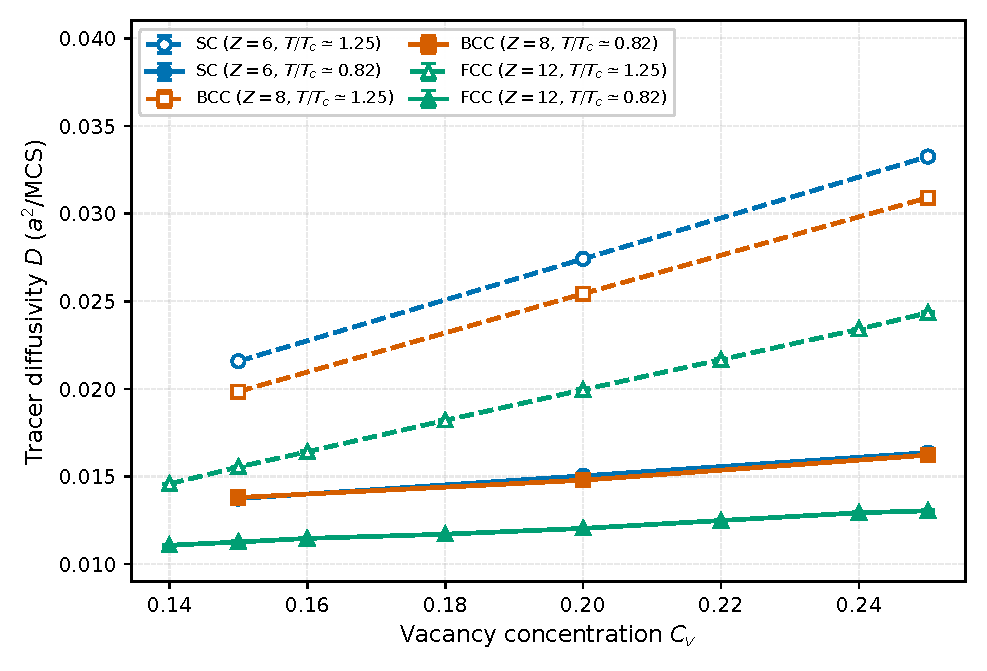
\includegraphics[width=\columnwidth]{fig02_diffusivity_vs_cv.pdf}
  \caption{\label{fig:diffusivity_vs_cv}Tracer diffusivity $D$ versus vacancy concentration $C_v$ at matched reduced temperatures $T/T_c \simeq 1.25$ (dashed lines, open markers) and $T/T_c \simeq 0.82$ (solid lines, filled markers), with $n = 15$ independent seeds per point ($\pm 1\;\mathrm{SE}$ error bars are smaller than the markers). Separating matched temperatures eliminates temperature-pooling bias and highlights both the thermal mobility boost across $T_c$ and the conventional-cell topology hierarchy of Eq.~\eqref{eq:dilute_exact}.}
\end{figure}

Dividing by $C_v$ at matched reduced temperatures exposes a sharp, fourfold contrast in the breakdown of independent-carrier scaling between the supercritical and subcritical regimes (Fig.~\ref{fig:norm_diffusivity}). Above $T_c$ ($T/T_c \simeq 1.25$), where vacancies remain only weakly clustered ($\mathcal{C} \approx 1.3$--$1.5$), $D/C_v$ declines gently across $C_v$: by $7.5\%$ in SC ($0.1438 \rightarrow 0.1330\;a^{2}/\mathrm{MCS}$ over $C_v = 0.15 \to 0.25$), $6.5\%$ in BCC ($0.1323 \rightarrow 0.1236$), and $6.5\%$ in FCC ($0.1041 \to 0.0974$ over $C_v = 0.14 \to 0.25$). Below $T_c$ ($T/T_c \simeq 0.82$), by contrast, strong attractive aggregation inside the miscibility gap depresses $D/C_v$ steeply: by $28.6\%$ in SC ($0.0916 \rightarrow 0.0654$), $29.5\%$ in BCC ($0.0920 \rightarrow 0.0649$), and $34.1\%$ in FCC ($0.0791 \rightarrow 0.0522$).

\begin{figure}[t]
  \centering
  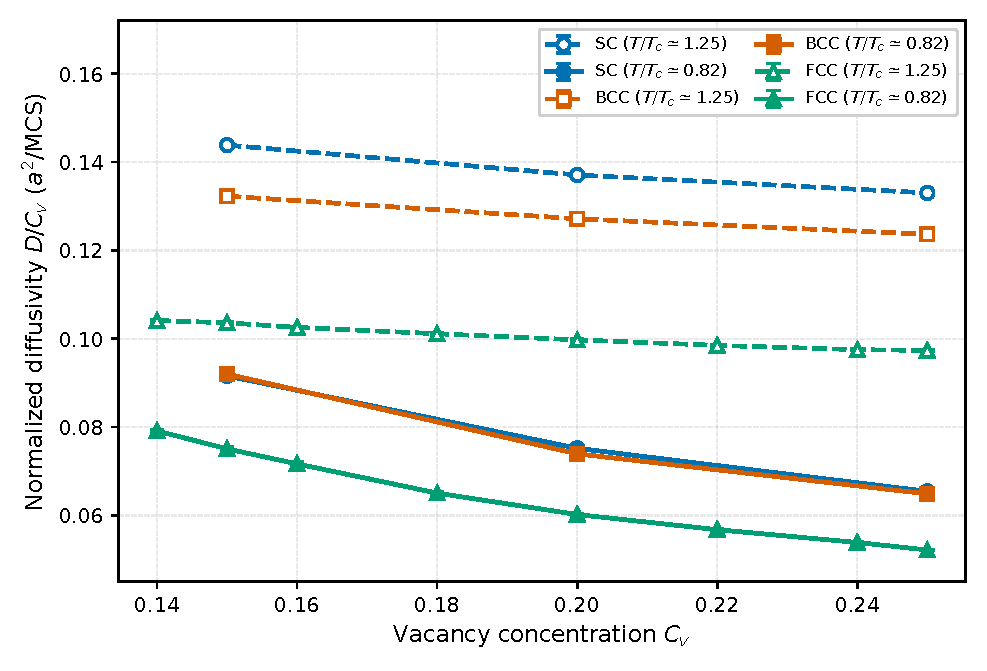
\includegraphics[width=\columnwidth]{fig03_normalized_diffusivity_vs_cv.pdf}
  \caption{\label{fig:norm_diffusivity}Normalized diffusivity $D/C_v$ versus $C_v$ at matched reduced temperatures $T/T_c \simeq 1.25$ (dashed, open markers) and $T/T_c \simeq 0.82$ (solid, filled markers; $n = 15$ seeds per point, $\pm 1\;\mathrm{SE}$). Below $T_c$, strong vacancy aggregation drives a $29\%$--$34\%$ drop in $D/C_v$, compared with a mild $6.5\%$--$7.5\%$ decrease above $T_c$.}
\end{figure}

\subsection{FCC Concentration Sweep, Finite-Time Spanning Crossovers, and $J=0$ Benchmarks}
\label{sec:fcc_sweep}

The dense canonical FCC concentration sweep ($C_v \in [0.14, 0.25]$, $n = 15$ seeds per point; complete numerical record in Table~\ref{tab:fcc_sweep_full}) resolves how macroscopic connectivity emerges across $p_c^{\mathrm{FCC}} = 0.1996$ (Fig.~\ref{fig:fcc_sweep}). Below $T_c$ ($T = 2.00$, $T/T_c = 0.816$), $f_{\max}$ climbs steadily from $22.1\%$ at $C_v = 0.14$ to $61.8\%$ at $C_v = 0.20$ and $78.8\%$ at $C_v = 0.25$. Comparing the subcritical ($T/T_c = 0.816$) and supercritical ($T/T_c = 1.249$) isotherms reveals a striking crossover near $C_v \approx 0.18$: for $C_v \le 0.16$, supercritical thermal disorder keeps vacancies fragmented ($f_{\max} \le 11.2\%$, $P_{\mathrm{span}} = 0$), whereas attractive demixing below $T_c$ forms substantial finite droplets ($f_{\max} = 22\%$--$33\%$). For $C_v \ge 0.20$, however, the supercritical curve \emph{surpasses} the subcritical curve, reaching $f_{\max} = 73.9\%$ ($P_{\mathrm{span}} = 1.00$) at $C_v = 0.20$ and $92.5\%$ at $C_v = 0.25$. Below $T_c$, strong attraction compacts vacancies into dense, locally enriched droplets ($\mathcal{C} = 2.39$ at $C_v = 0.20$) whose slow conserved coarsening leaves disconnected droplets at $6{,}000$ MCS; above $T_c$, thermal agitation disperses compact droplets into a space-filling, weakly correlated ($\mathcal{C} = 1.30$) network stabilized by twelve-fold coordination and residual attraction.

\begin{figure}[t]
  \centering
  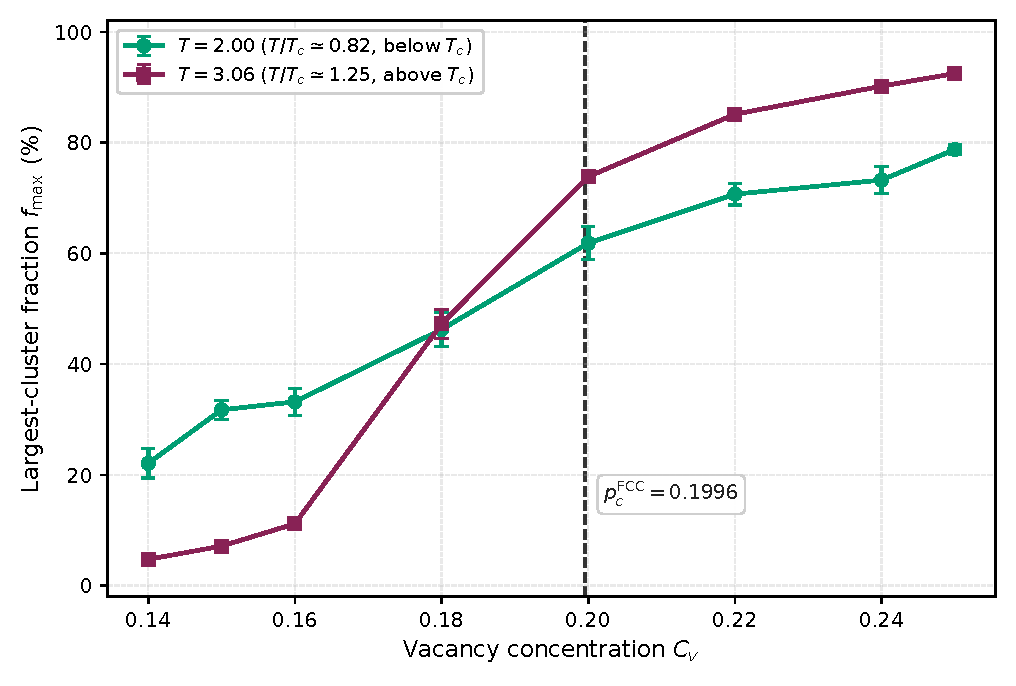
\includegraphics[width=\columnwidth]{fig04_fcc_giant_cluster_vs_cv.pdf}
  \caption{\label{fig:fcc_sweep}FCC largest-cluster fraction $f_{\max}$ (\%) across $C_v \in [0.14, 0.25]$ (canonical $n = 15$ seeds per point; error bars show $\pm 1\;\mathrm{SE}$) below $T_c$ ($T=2.00$, $T/T_{\mathrm c} \simeq 0.82$) and above $T_c$ ($T=3.06$, $T/T_{\mathrm c} \simeq 1.25$). The two isotherms intersect near $C_v \approx 0.18$: thermal disorder fragments clusters below $p_c^{\mathrm{FCC}}$, whereas above $p_c^{\mathrm{FCC}}$ it disperses compact droplets into a space-filling percolating mesh with larger $f_{\max}$.}
\end{figure}

To quantify finite-time spanning crossovers with tight statistical confidence and isolate finite-size effects from interaction effects, Fig.~\ref{fig:spanning} and Table~\ref{tab:spanning} compare our non-interacting ($J = 0$) random site-percolation benchmarks ($n = 200$/point at $L = 20$; $n = 100$/point at $L = 30, 40$) directly against our high-precision interacting ($J = 1$) finite-time crossover sweeps at $6{,}000$ MCS ($n = 50$ seeds/point across every transition window, fitted via exact binomial logistic MLE with $2{,}000$-resample bootstrap $95\%$ CIs).

First, the $J = 0$ benchmarks confirm that our periodic wrapping algorithm reproduces the infinite-lattice random thresholds $p_c$ on $L = 20$ supercells to within $0.1\%$--$0.6\%$: $C_v^{*,J=0} = 0.3119$ ($95\%$ CI $[0.3109, 0.3127]$, $1.001\,p_c^{\mathrm{SC}}$) for SC, $0.2469$ ($[0.2461, 0.2476]$, $1.006\,p_c^{\mathrm{BCC}}$) for BCC, and $0.1992$ ($[0.1988, 0.1997]$, $0.998\,p_c^{\mathrm{FCC}}$) for FCC, sharpening smoothly with system size across $L = 30$ ($0.1992$, $\gamma_1 = 399$) and $L = 40$ ($0.1994$ $[0.1990, 0.1997]$, $\gamma_1 = 613$). Finite-size shifts of uncorrelated random percolation at $L = 20$ are therefore negligible ($< 0.6\%$) compared with the large shifts produced by attractive interactions and conserved kinetics.

Second, at matched subcritical temperature ($T/T_c \simeq 0.82$, $J = 1$, $6{,}000$ MCS), finite-time spanning crossover concentrations normalized by either $p_c$ or $C_v^{*,J=0}(L=20)$ reveal a four-part thermodynamic-to-geometric progression (Table~\ref{tab:spanning}). The crossover estimates and their confidence intervals are reported separately for each lattice and regime:
\begin{itemize}
  \item \textbf{SC ($Z = 6$, below $T_c$):} $C_v^* = 0.2148$ ($95\%$ CI $[0.2099, 0.2206]$), giving $C_v^*/p_c^{\mathrm{SC}} = 0.689$ ($[0.674, 0.708]$) and $C_v^{*,J=1}/C_v^{*,J=0} = 0.689$ ($[0.673, 0.707]$)---thermodynamic aggregation advances finite-time spanning $31.1\%$ below the random percolation benchmark.
  \item \textbf{BCC ($Z = 8$, below $T_c$):} $C_v^* = 0.2175$ ($[0.2114, 0.2228]$), giving $C_v^*/p_c^{\mathrm{BCC}} = 0.886$ ($[0.861, 0.907]$) and $C_v^{*,J=1}/C_v^{*,J=0} = 0.881$ ($[0.856, 0.902]$)---an intermediate downward shift $11.9\%$ below $C_v^{*,J=0}$.
  \item \textbf{FCC ($Z = 12$, below $T_c$):} $C_v^* = 0.2083$ ($[0.2045, 0.2125]$), giving $C_v^*/p_c^{\mathrm{FCC}} = 1.044$ ($[1.024, 1.065]$) and $C_v^{*,J=1}/C_v^{*,J=0} = 1.046$ ($[1.026, 1.067]$). Crucially, the $95\%$ confidence interval strictly \emph{excludes} unity: compact droplet aggregation actually \emph{delays} finite-time system-wide wrapping slightly above the random geometric reference because local vacancy sequestration ($\mathcal{C} \approx 2.38$) leaves disconnected droplets and pinches off inter-droplet bridges over $6{,}000$ MCS (confirmed directly by the coarsening trajectories in Sec.~\ref{sec:finite_size}).
  \item \textbf{FCC ($Z = 12$, above $T_c$):} Heating to $T/T_c = 1.249$ shifts the spanning crossover \emph{below} the random benchmark again, to $C_v^* = 0.1761$ ($[0.1747, 0.1775]$), or $0.882\,p_c^{\mathrm{FCC}}$ ($0.884\,C_v^{*,J=0}$), quantifying an $11.6\%$ downward shift driven by residual supercritical short-range correlations ($\mathcal{C} \approx 1.31$--$1.33$).
\end{itemize}
Sensitivity fits restricted strictly to the uniform $n = 50$ transition windows reproduce identical values within $0.0003$--$0.0029$ (SC $0.2156$, BCC $0.2179$, FCC below $T_c$ $0.2112$, FCC above $T_c$ $0.1761$). Throughout, these $C_v^*$ values represent finite-time spanning crossover concentrations at $6{,}000$ MCS under conserved dynamics rather than equilibrium critical percolation thresholds.

\begin{figure*}[t]
  \centering
  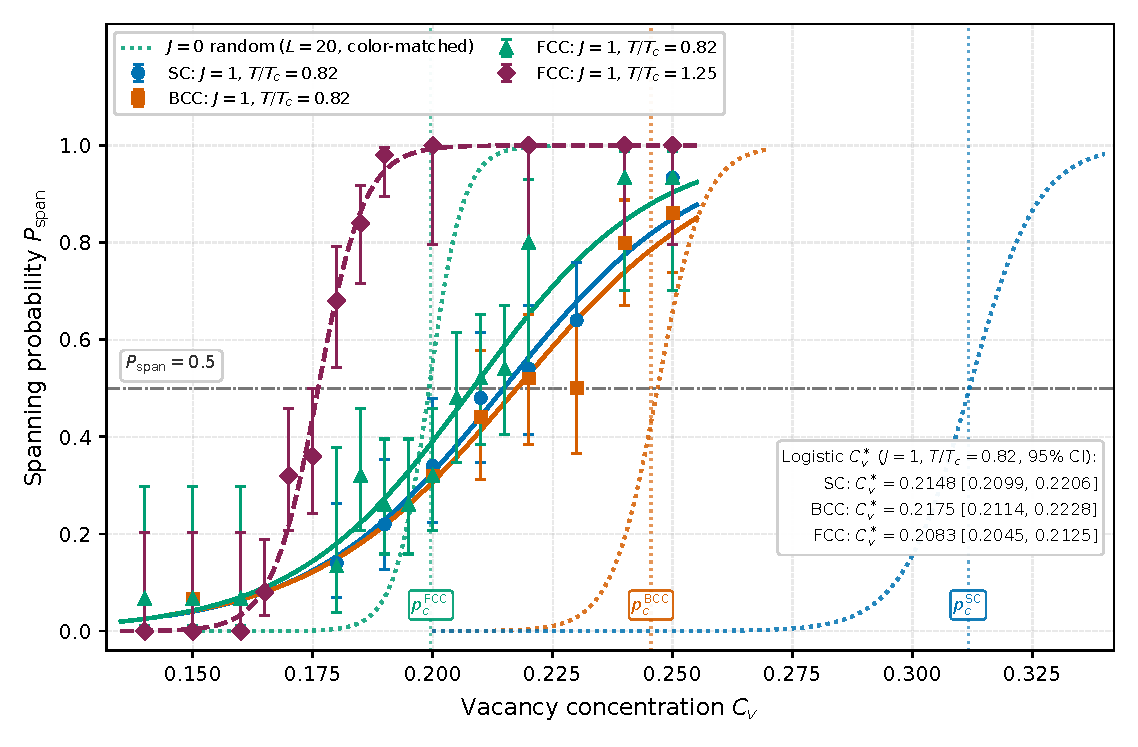
\includegraphics[width=0.80\textwidth]{fig05_spanning_probability_crossover.pdf}
  \caption{\label{fig:spanning}Exact periodic spanning probability $P_{\mathrm{span}}$ versus $C_v$ with $95\%$ Wilson binomial confidence intervals and binomial logistic MLE fits for interacting ($J = 1$) systems at $6{,}000$ MCS at matched subcritical $T/T_c \simeq 0.82$ (solid curves; $n = 50$ seeds/point across each transition window plus $n = 15$ canonical outer points) and supercritical FCC ($T/T_c = 1.25$, dashed curve), compared directly with color-matched non-interacting ($J = 0$, $L = 20$, $n = 200$/point) random site-percolation logistic curves (dotted) and infinite-lattice $p_c$ (vertical lines). Relative to $J = 0$, subcritical finite-time spanning shifts downward relative to the $J=0$ finite-size baseline in SC ($0.689$) and BCC ($0.881$). In subcritical FCC, the crossover lies at $1.044\,p_c^{\mathrm{FCC}}$, corresponding to a ratio of $1.046$ relative to the finite-size $J=0$ crossover. In supercritical FCC, it shifts below the random reference to $0.882\,p_c^{\mathrm{FCC}}$ (a ratio of $0.884$ relative to the $J=0$ finite-size crossover). For BCC, the ratio to the infinite-lattice threshold is $0.886$; the ratio to the finite-size $J=0$ crossover is $0.881$.}
\end{figure*}

\begin{table*}[t]
\caption{\label{tab:spanning}Binomial logistic-regression MLE finite-time spanning crossover concentrations $C_v^*$ ($P_{\mathrm{span}} = 0.5$) with $2{,}000$-resample stratified bootstrap $95\%$ confidence intervals for non-interacting ($J = 0$) random site percolation ($n = 200$/point at $L = 20$; $n = 100$/point at $L = 30, 40$) and interacting ($J = 1$, $L = 20$, $6{,}000$ MCS) ensembles combining the $n = 50$/point high-precision transition windows with $n = 15$ canonical outer-tail points (total realizations $N_{\mathrm{tot}}$ listed; distinct from the $n = 15$ matched-temperature control ensembles in Table~\ref{tab:thermo_controls}). Columns give logistic $C_v^*$, its ratio to the infinite-lattice $p_c$, the bootstrap ratio $C_v^{*,J=1}/C_v^{*,J=0}(L=20)$, and the logistic slope $\gamma_1$.}
\begingroup
\footnotesize
\setlength{\tabcolsep}{4pt}
\begin{ruledtabular}
\begin{tabular}{lccccccc}
System / Regime & $L$ & $T/T_c$ & $N_{\mathrm{tot}}$ & $C_v^*$ [$95\%$ CI] & $C_v^*/p_c$ [$95\%$ CI] & $C_v^{*,J=1}/C_v^{*,J=0}$ [$95\%$ CI] & $\gamma_1$ \\
\colrule
SC ($J=0$)  & $20$ & --- & $2{,}400$ & $0.3119$ [$0.3109,0.3127$] & $1.001$ [$0.998,1.004$] & --- & $142.0$ \\
BCC ($J=0$) & $20$ & --- & $2{,}000$ & $0.2469$ [$0.2461,0.2476$] & $1.006$ [$1.003,1.008$] & --- & $208.8$ \\
FCC ($J=0$) & $20$ & --- & $2{,}400$ & $0.1992$ [$0.1988,0.1997$] & $0.998$ [$0.996,1.000$] & --- & $280.7$ \\
FCC ($J=0$) & $30$ & --- & $700$     & $0.1992$ [$0.1987,0.1998$] & $0.998$ [$0.996,1.001$] & --- & $399.0$ \\
FCC ($J=0$) & $40$ & --- & $700$     & $0.1994$ [$0.1990,0.1997$] & $0.999$ [$0.997,1.001$] & --- & $612.8$ \\
\colrule
SC ($J=1$, $T=0.93$)  & $20$ & $0.823$ & $330$ & $0.2148$ [$0.2099,0.2206$] & $0.689$ [$0.674,0.708$] & $0.689$ [$0.673,0.707$] & $49.0$ \\
BCC ($J=1$, $T=1.30$) & $20$ & $0.818$ & $315$ & $0.2175$ [$0.2114,0.2228$] & $0.886$ [$0.861,0.907$] & $0.881$ [$0.856,0.902$] & $46.4$ \\
FCC ($J=1$, $T=2.00$) & $20$ & $0.816$ & $455$ & $0.2083$ [$0.2045,0.2125$] & $1.044$ [$1.024,1.065$] & $1.046$ [$1.026,1.067$] & $53.5$ \\
FCC ($J=1$, $T=3.06$) & $20$ & $1.249$ & $405$ & $0.1761$ [$0.1747,0.1775$] & $0.882$ [$0.875,0.890$] & $0.884$ [$0.877,0.892$] & $208.9$ \\
\end{tabular}
\end{ruledtabular}
\endgroup
\end{table*}

\subsection{Matched Reduced-Temperature Controls and Three-Way FCC Isolation}
\label{sec:thermo_controls}

To separate thermodynamic aggregation, uncorrelated percolation geometry, and residual supercritical correlations directly, Table~\ref{tab:thermo_controls} and Fig.~\ref{fig:thermo_controls} contrast matched reduced temperatures below ($T/T_c \simeq 0.82$) and above ($T/T_c \simeq 1.25$) each lattice's critical point ($n = 15$ canonical seeds per condition) alongside the exact non-interacting ($J = 0$, $n = 200$) $L = 20$ baseline and the expanded $n = 50$ subcritical FCC $C_v = 0.20$ sample.

At $C_v = 0.20$, heating SC ($C_v/p_c = 0.642$) above $T_c$ collapses $f_{\max}$ from $66.5 \pm 3.0\%$ to $12.5 \pm 5.7\%$ (Welch $t = 32.46$, $p = 1.28 \times 10^{-19}$; $P_{\mathrm{span}}$ dropping from $0.467$ to $0.067$), confirming thermodynamically driven aggregation far below random percolation ($J = 0$ SC gives $f_{\max} = 2.2\%$, $P_{\mathrm{span}} = 0$). Heating BCC ($C_v/p_c = 0.815$) likewise reduces vacancy aggregation substantially ($f_{\max} = 63.6 \pm 6.9\% \to 40.8 \pm 10.5\%$, $t = 7.03$, $p = 2.77 \times 10^{-7}$); however, rather than completely dissolving, supercritical BCC retains substantial connected structures ($f_{\max} = 40.8\%$, $P_{\mathrm{span}} = 0.333$, $95\%$ Wilson CI $[0.152, 0.583]$) compared with its uncorrelated $J = 0$ baseline ($f_{\max} = 3.7\%$, $P_{\mathrm{span}} = 0.000$), because $C_v/p_c^{\mathrm{BCC}} = 0.815$ lies close enough to $p_c^{\mathrm{BCC}}$ that residual supercritical attraction ($\mathcal{C} = 1.40$) creates partial percolating paths.

\begin{figure*}[t]
  \centering
  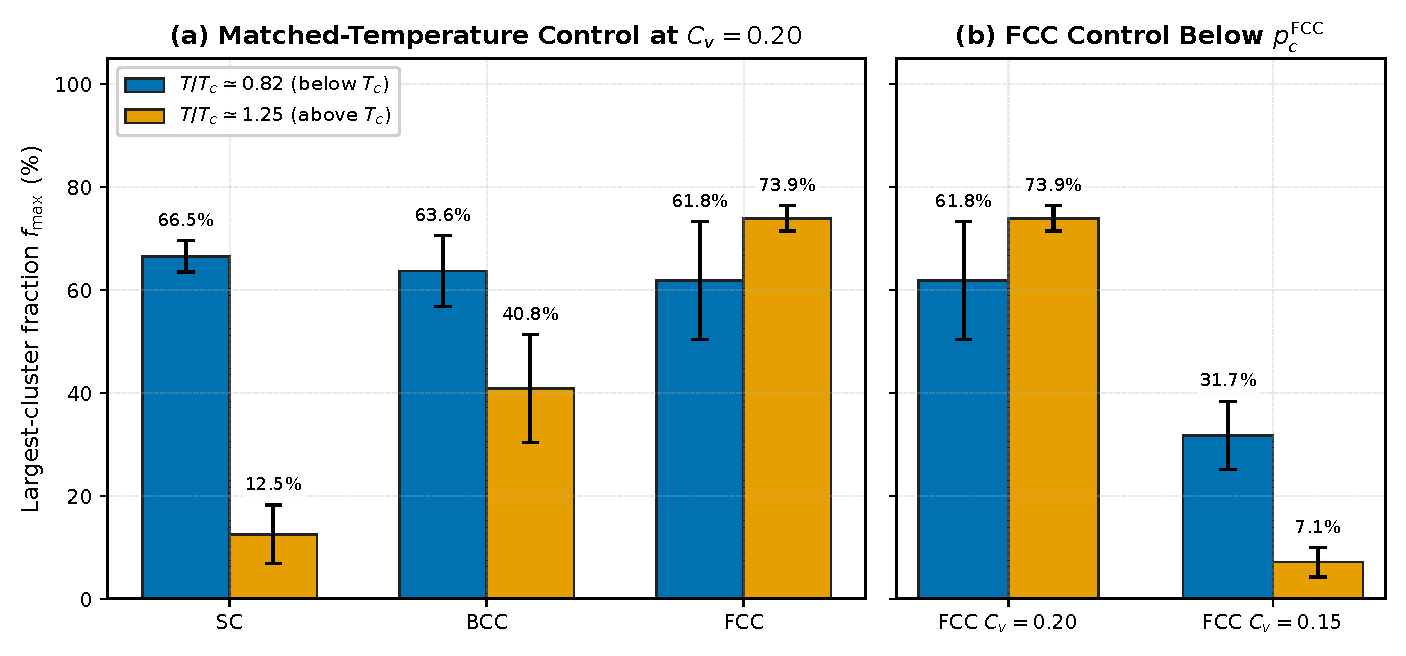
\includegraphics[width=0.92\textwidth]{fig06_thermo_controls_cv020.pdf}
  \caption{\label{fig:thermo_controls}Matched reduced-temperature controls (canonical $n = 15$ seeds per bar; error bars show $\pm 1\;\mathrm{SD}$). (a) At $C_v = 0.20$, heating from $T/T_c \simeq 0.82$ to $1.25$ strongly suppresses $f_{\max}$ in SC ($66.5\% \to 12.5\%$) and substantially reduces it in BCC ($63.6\% \to 40.8\%$, where partial connectivity persists), whereas FCC retains and expands its spanning network ($61.8\% \to 73.9\%$, $P_{\mathrm{span}} = 1.00$). (b) Reducing FCC to $C_v = 0.15 < p_c^{\mathrm{FCC}}$ restores strong thermal suppression ($31.7\% \to 7.1\%$). All bar heights and uncertainties match the canonical $n = 15$ entries of Table~\ref{tab:thermo_controls} identically.}
\end{figure*}

\begin{table*}[t]
\caption{\label{tab:thermo_controls}Matched reduced-temperature control summary at $L = 20$ comparing non-interacting random placement ($J = 0$, $n = 200$) with canonical interacting runs ($J = 1$, $6{,}000$ MCS, $n = 15$ per condition) below ($T/T_c \simeq 0.82$) and above ($T/T_c \simeq 1.25$) $T_c$; the precise lattice-specific reduced temperatures are given in the Methods section. The table also includes the expanded $n = 50$ subcritical FCC sample at $C_v = 0.20$. Reported are ensemble mean $\pm$ SD for $f_{\max}$, spanning probability $P_{\mathrm{span}}$ [$95\%$ Wilson CI], mean local clustering $\mathcal{C}$, mean diffusivity $D$ (in $10^{-2}\,a^2/\mathrm{MCS}$), and two-sided Welch $t$-tests comparing canonical ($n = 15$) $f_{\max}$ below versus above $T_c$.}
\begingroup
\footnotesize
\setlength{\tabcolsep}{4pt}
\begin{ruledtabular}
\begin{tabular}{lclcccccc}
Lat. & $C_v$ & Regime & $n$ & $f_{\max}$ (\%) & $P_{\mathrm{span}}$ [95\% CI] & $\mathcal{C}$ & $D$ ($10^{-2}$) & Welch $t$ ($p$) \\
\colrule
SC  & $0.20$ & $J=0$ random         & $200$ & $2.2 \pm 0.7$   & $0.000$ [$0.00,0.02$] & $1.00$ & ---     & --- \\
SC  & $0.20$ & $J=1$, subcrit. & $15$  & $66.5 \pm 3.0$  & $0.467$ [$0.25,0.70$] & $2.57$ & $1.504$ & --- \\
SC  & $0.20$ & $J=1$, supercrit. & $15$  & $12.5 \pm 5.7$  & $0.067$ [$0.01,0.30$] & $1.56$ & $2.741$ & $32.46$ ($1.28 \times 10^{-19}$) \\
\colrule
BCC & $0.20$ & $J=0$ random         & $200$ & $3.7 \pm 1.4$   & $0.000$ [$0.00,0.02$] & $1.00$ & ---     & --- \\
BCC & $0.20$ & $J=1$, subcrit. & $15$  & $63.6 \pm 6.9$  & $0.267$ [$0.11,0.52$] & $2.46$ & $1.479$ & --- \\
BCC & $0.20$ & $J=1$, supercrit. & $15$  & $40.8 \pm 10.5$ & $0.333$ [$0.15,0.58$] & $1.40$ & $2.543$ & $7.03$ ($2.77 \times 10^{-7}$) \\
\colrule
FCC & $0.20$ & $J=0$ random         & $200$ & $33.3 \pm 11.2$ & $0.480$ [$0.41,0.55$] & $1.00$ & ---     & --- \\
FCC & $0.20$ & $J=1$, subcrit. (canon.) & $15$ & $61.8 \pm 11.5$ & $0.467$ [$0.25,0.70$] & $2.39$ & $1.204$ & --- \\
FCC & $0.20$ & $J=1$, subcrit. (high-$n$) & $50$ & $59.9 \pm 11.6$ & $0.320$ [$0.21,0.46$] & $2.38$ & $1.204$ & --- \\
FCC & $0.20$ & $J=1$, supercrit. & $15$  & $73.9 \pm 2.4$  & $1.000$ [$0.80,1.00$] & $1.30$ & $1.995$ & $-3.96$ ($1.21 \times 10^{-3}$) \\
\colrule
FCC & $0.15$ & $J=0$ random         & $200$ & $2.0 \pm 0.6$   & $0.000$ [$0.00,0.02$] & $1.00$ & ---     & --- \\
FCC & $0.15$ & $J=1$, subcrit. & $15$  & $31.7 \pm 6.7$  & $0.067$ [$0.01,0.30$] & $2.15$ & $1.126$ & --- \\
FCC & $0.15$ & $J=1$, supercrit. & $15$  & $7.1 \pm 2.9$   & $0.000$ [$0.00,0.20$] & $1.32$ & $1.554$ & $13.11$ ($5.36 \times 10^{-11}$) \\
\end{tabular}
\end{ruledtabular}
\endgroup
\end{table*}

In sharp contrast, heating FCC at $C_v = 0.20$ ($C_v/p_c^{\mathrm{FCC}} = 1.002$) \emph{enlarges} the giant cluster significantly from $f_{\max} = 61.8 \pm 11.5\%$ ($59.9 \pm 11.6\%$ across $n = 50$) to $73.9 \pm 2.4\%$ ($p = 1.21 \times 10^{-3}$) and drives $P_{\mathrm{span}}$ to $1.000$ ($95\%$ Wilson CI $[0.796, 1.000]$) even as local clustering drops from $\mathcal{C} = 2.39$ to $1.30$ and diffusivity increases by $66\%$ ($0.01204 \to 0.01995\;a^2/\mathrm{MCS}$). Directly comparing all three FCC regimes at $C_v = 0.20$ (Fig.~\ref{fig:fcc_3way} and Table~\ref{tab:thermo_controls}) cleanly isolates the respective roles of lattice geometry and attractive interactions:
\begin{enumerate}
  \item \textbf{Non-interacting random ($J = 0$, $\mathcal{C} = 1.00$):} Places FCC directly on the critical geometric percolation edge, with $f_{\max} = 33.3 \pm 11.2\%$ and $P_{\mathrm{span}} = 0.480$ ($[0.412, 0.549]$)---spanning occurs in less than half of realizations [Fig.~\ref{fig:fcc_3way}(c)].
  \item \textbf{Supercritical interacting ($J = 1, T/T_c = 1.25$, $\mathcal{C} = 1.30$):} Introducing attractive interactions above $T_c$ creates residual short-range correlations that lift $f_{\max}$ from $33.3\%$ to $73.9\%$ and $P_{\mathrm{span}}$ from $0.480$ to $1.000$, turning the critical threshold into a space-filling spanning backbone [Fig.~\ref{fig:fcc_3way}(b)].
  \item \textbf{Subcritical interacting ($J = 1, T/T_c = 0.82$, $\mathcal{C} = 2.38$--$2.39$):} Strong attraction pulls vacancies into compact, locally enriched coarsening droplets that reduce spatial reach relative to the supercritical mesh ($f_{\max} = 59.9\%$--$61.8\%$, $P_{\mathrm{span}} = 0.320$ for $n = 50$) [Fig.~\ref{fig:fcc_3way}(a)].
\end{enumerate}
Lowering FCC to $C_v = 0.15$ ($C_v/p_c^{\mathrm{FCC}} = 0.752 < 1$) removes this geometric proximity and restores decisive thermal destruction ($f_{\max} = 31.7 \pm 6.7\% \to 7.1 \pm 2.9\%$, $p = 5.36 \times 10^{-11}$, $P_{\mathrm{span}} = 0$; Fig.~\ref{fig:thermo_controls}(b)). Thus, FCC geometry provides a highly connected framework, while residual attractive interactions substantially enhance the formation of a system-spanning vacancy network above the thermodynamic ordering temperature.

\begin{figure*}[t]
  \centering
  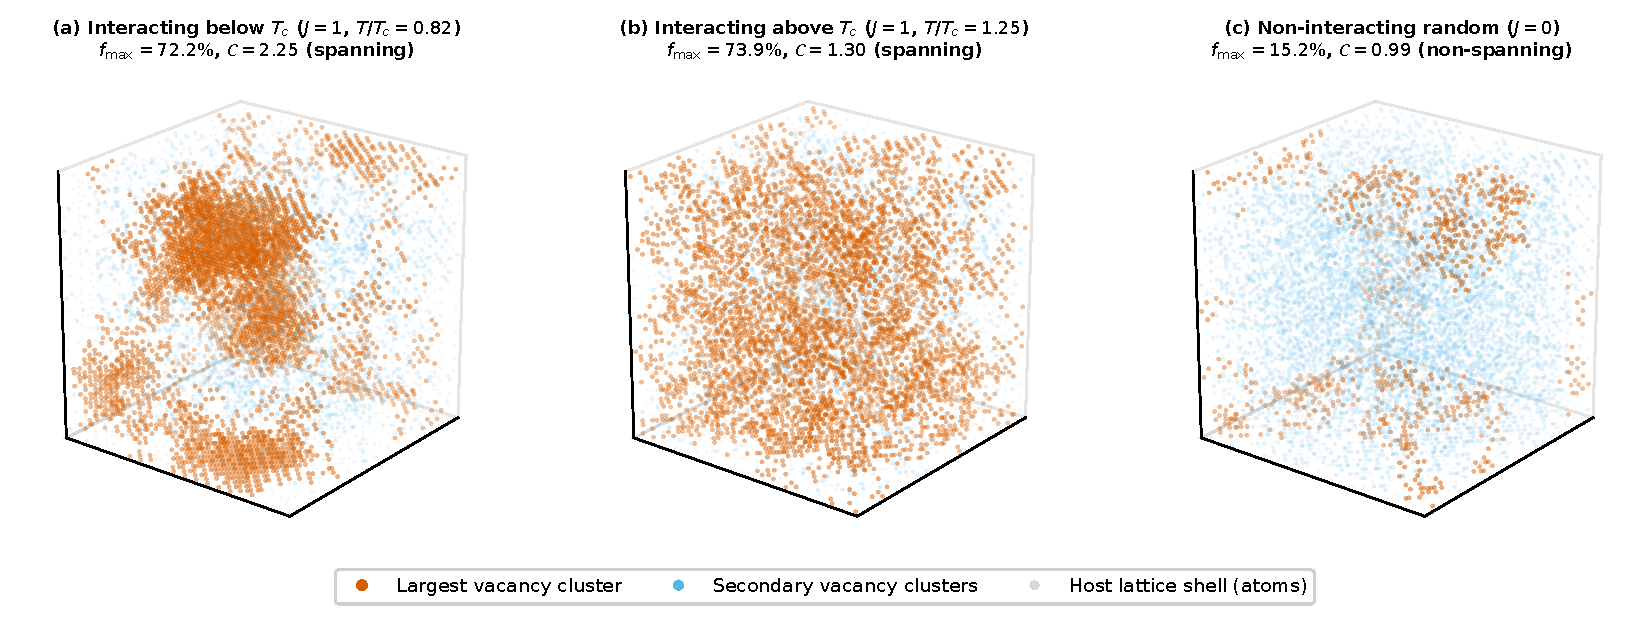
\includegraphics[width=0.98\textwidth]{fig06b_fcc_3way_morphology.pdf}
  \caption{\label{fig:fcc_3way}Three-way $3\mathrm{D}$ morphological comparison for FCC at $C_v = 0.20$ ($L = 20$, $N = 32{,}000$, $N_v = 6{,}400$ vacancies; deterministic seed index $0$). (a) Interacting below $T_c$ ($J = 1$, $T/T_c = 0.82$, $6{,}000$ MCS): compact, locally enriched coarsening droplets ($\mathcal{C} = 2.25$ in this realization; ensemble $\mathcal{C} = 2.38$). (b) Interacting above $T_c$ ($J = 1$, $T/T_c = 1.25$, $6{,}000$ MCS): dispersed, space-filling correlated spanning mesh ($\mathcal{C} = 1.30$, $f_{\max} = 73.9\%$, ensemble $P_{\mathrm{span}} = 1.00$). (c) Non-interacting random placement ($J = 0$): uncorrelated percolation baseline right at $p_c^{\mathrm{FCC}}$ ($\mathcal{C} = 0.99$, ensemble $f_{\max} = 33.3\%$, $P_{\mathrm{span}} = 0.480$). Colors follow Fig.~\ref{fig:snapshots}.}
\end{figure*}

\subsection{Local Clustering vs.\ Global Connectivity: Covariate Control and Condition Fixed Effects}
\label{sec:structure_transport}

Across all $465$ canonical seed-level trajectories, production-window local clustering $\bar{\mathcal{C}}$ (averaged over all $25$ MSD checkpoints across $[2{,}000, 6{,}000]$ MCS) tracks final $\mathcal{C}(6{,}000)$ tightly ($r = 0.9934$, mean difference $\mathcal{C} - \bar{\mathcal{C}} = +0.038$, mean within-window $\mathrm{SD} = 0.049$), confirming modest late-stage drift during MSD accumulation. Table~\ref{tab:struct_transport} evaluates $f_{\max}$, final $\mathcal{C}$, and time-aligned $\bar{\mathcal{C}}$ using three levels of statistical control: bivariate correlation, parametric covariate-controlled multiple OLS [Eq.~\eqref{eq:controlled_ols}], and linear condition-fixed-effects regression [Eq.~\eqref{eq:condition_fe}].

Bivariately, macroscopic cluster size $f_{\max}$ fails as a transport coordinate: pooled linear ($r = -0.089$, $p = 0.056$) and rank ($\rho = -0.031$, $p = 0.510$) correlations are negligible, log--log regression yields $R^2 = 0.026$, and individual lattices display \emph{opposite} signs (negative in SC, $r = -0.382$; positive in BCC, $+0.241$, and FCC, $+0.497$). By contrast, the time-aligned clustering measure $\bar{\mathcal{C}}$ is strongly and negatively associated with $D$ across every topology ($r = -0.651$, $p = 2.48 \times 10^{-57}$; $\rho = -0.612$, $p = 4.40 \times 10^{-49}$; within-lattice $r \in [-0.889, -0.800]$; Fig.~\ref{fig:d_vs_c}), matching final $\mathcal{C}$ ($r = -0.656$, $p = 1.42 \times 10^{-58}$).

\begin{figure}[t]
  \centering
  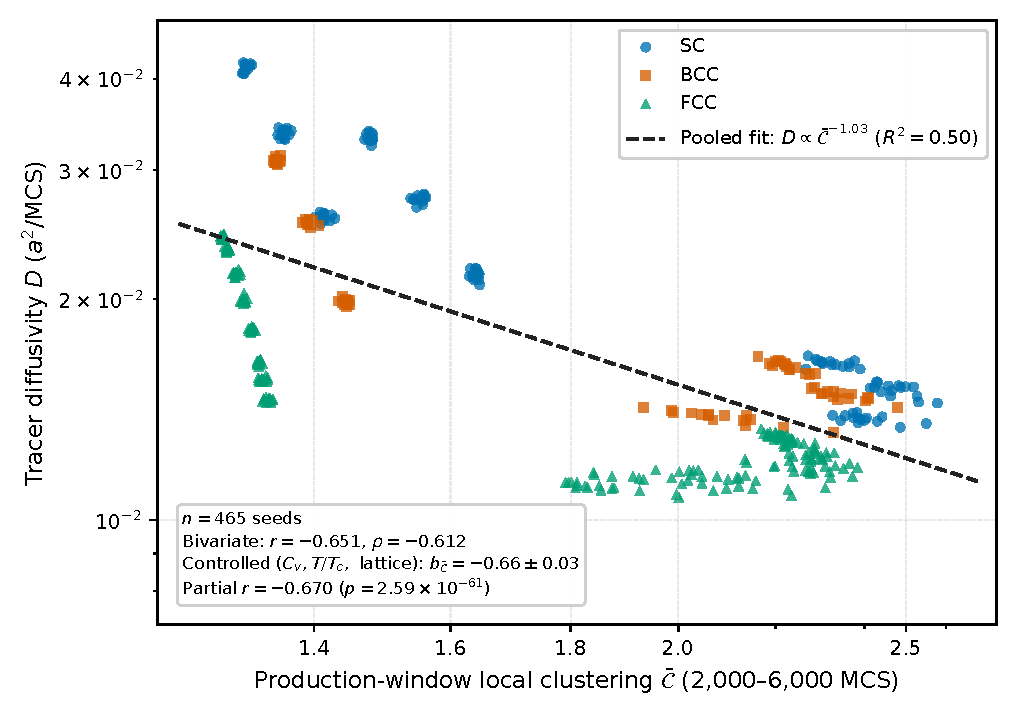
\includegraphics[width=\columnwidth]{fig07_diffusivity_vs_clustering.pdf}
  \caption{\label{fig:d_vs_c}Seed-level tracer diffusivity $D$ versus production-window local clustering index $\bar{\mathcal{C}}$ (averaged over $2{,}000$--$6{,}000$ MCS) across all $n = 465$ canonical trajectories. Higher local clustering is negatively associated with diffusivity bivariately ($r=-0.651$, $\rho=-0.612$) and under linear covariate control ($b_{\bar{\mathcal{C}}}=-0.664\pm0.034$, partial $r=-0.670$, $p=2.59\times10^{-61}$). Within identical fixed $(C_v,T,\text{lattice})$ conditions, the association is strong overall ($R^2_{\mathrm{within}}=0.495$, wild-bootstrap $p=0.0001$) and is concentrated in the subcritical regime.}
\end{figure}

In the covariate-controlled OLS model [Eq.~\eqref{eq:controlled_ols}], adding time-aligned $\ln\bar{\mathcal{C}}$ to the $(\ln C_v, \ln(T/T_c), \text{lattice})$ baseline ($R^2_{\log} = 0.9584$) raises $R^2_{\log}$ to $0.9771$ ($\Delta R^2 = +0.0187$), accounting for $44.9\%$ of all residual log-variance ($b_{\bar{\mathcal{C}}} = -0.664 \pm 0.034$, partial $r = -0.670$, $p = 2.59 \times 10^{-61}$, $F(1,459) = 373.4$). Allowing lattice-specific $\ln\bar{\mathcal{C}}$ slopes further raises $R^2_{\log}$ to $0.9861$ ($F(2,457) = 147.8$, $p = 3.09 \times 10^{-50}$), with strongly negative controlled slopes in every lattice ($-1.287 \pm 0.064$ SC, $-1.029 \pm 0.093$ BCC, $-0.939 \pm 0.050$ FCC).

The \emph{condition-fixed-effects} \mbox{regression} [Eq.~\eqref{eq:condition_fe}] controls for arbitrary additive differences among the $G=31$ fixed $(C_v,T,\text{lattice})$ conditions ($N=465$ seeds). Its slope is estimated from seed-to-seed variation within each condition, testing whether independent trajectories at identical temperature, concentration, and lattice that develop higher local clustering also exhibit lower diffusivity (Table~\ref{tab:struct_transport}, Panel B):
\begin{itemize}
  \item \textbf{Time-aligned $\bar{\mathcal{C}}_{ij} - \overline{\bar{\mathcal{C}}}_j$:} Yields $\hat{\beta}_{\mathrm{FE}} = -0.2040$ with condition-clustered $\mathrm{SE}_{\mathrm{CR1}} = 0.0132$ ($t_{30} = -15.49$, $p_{\mathrm{CR1}} = 7.49 \times 10^{-16}$) and $9{,}999$-draw Rademacher wild cluster bootstrap $p_{\mathrm{WCB}} = 0.0001$ ($95\%$ CI $[-0.2278, -0.1800]$), accounting for $R^2_{\mathrm{within}} = 0.4949$ ($r_{\mathrm{within}} = -0.7035$)---nearly half of all within-condition seed-to-seed $\ln D$ variance! The centered log specification ($\ln\bar{\mathcal{C}}_{ij} - \overline{\ln\bar{\mathcal{C}}}_j$) yields the same strong association ($\hat{\beta}_{\mathrm{FE}} = -0.4280 \pm 0.0334$, $t_{30} = -12.82$, $p_{\mathrm{CR1}} = 1.06 \times 10^{-13}$, $p_{\mathrm{WCB}} = 0.0001$, $R^2_{\mathrm{within}} = 0.4804$).
  \item \textbf{Subcritical vs.\ supercritical decomposition:} Restricting Eq.~\eqref{eq:condition_fe} (in identical centered linear form $\bar{\mathcal{C}}_{ij} - \overline{\bar{\mathcal{C}}}_j$) to the $14$ subcritical conditions ($N = 210$), where conserved coarsening generates genuine seed-to-seed clustering heterogeneity, boosts within-condition explanatory power to $R^2_{\mathrm{within}} = 0.6795$ ($r_{\mathrm{within}} = -0.8243$, $\hat{\beta}_{\mathrm{FE}} = -0.2054 \pm 0.0138$, $t_{13} = -14.94$, $p_{\mathrm{CR1}} = 1.45 \times 10^{-9}$, $p_{\mathrm{WCB}} = 0.0003$). Across the $17$ supercritical conditions ($N=255$), where sampled trajectories fluctuate within a narrow range around their condition-specific means ($\mathrm{SD}(\bar{\mathcal{C}}) \lesssim 0.006$), the same centered linear specification yields no statistically detectable within-condition association ($\hat{\beta}_{\mathrm{FE}} = +0.0689 \pm 0.1452$, $R^2_{\mathrm{within}} = 0.0011$, $p_{\mathrm{CR1}} = 0.642$, $p_{\mathrm{WCB}} = 0.636$).
  \item \textbf{Final $\mathcal{C}(6{,}000)$ vs.\ window $\bar{\mathcal{C}}$:} Replacing time-aligned $\bar{\mathcal{C}}$ with final-snapshot $\ln\mathcal{C}$ cuts within-condition $R^2_{\mathrm{within}}$ by more than half (from $0.4804$ to $0.2083$, $r_{\mathrm{within}} = -0.4564$), directly validating window-averaged alignment.
  \item \textbf{Global $f_{\max}$ completely null:} Under condition fixed effects, the small positive artifact seen for $\ln f_{\max}$ under linear covariate control vanishes completely: $f_{\max,ij} - \bar{f}_{\max,j}$ yields $\hat{\beta}_{\mathrm{FE}} = -0.0118 \pm 0.0116$ ($t_{30} = -1.02$, $p_{\mathrm{CR1}} = 0.317$, $p_{\mathrm{WCB}} = 0.309$, $R^2_{\mathrm{within}} = 0.0044$), and centered $\ln f_{\max}$ likewise gives $R^2_{\mathrm{within}} = 0.0051$ ($p_{\mathrm{WCB}} = 0.209$).
\end{itemize}
We interpret these results carefully as a strong conditional association between local vacancy coordination and diffusivity---mechanistically supported by the exact atom--vacancy interface identity Eq.~\eqref{eq:bond_conservation}---rather than proof that local clustering alone causally determines diffusivity, since Metropolis activation barriers and tracer correlation factors jointly mediate microscopic jump kinetics~\cite{Kehr1984,Kehr1989}.

\begin{table*}[t]
\caption{\label{tab:struct_transport}Structure--transport diagnostics across all $n = 465$ canonical trajectories ($n_{\mathrm{SC}} = 135$, $n_{\mathrm{BCC}} = 90$, $n_{\mathrm{FCC}} = 240$). Panel A reports bivariate correlations ($D$ vs.\ $X$) and parametric covariate-controlled OLS [Eq.~\eqref{eq:controlled_ols}, adjusting for $\ln C_v$, $\ln(T/T_c)$, and lattice; baseline $R^2_{\log} = 0.9584$]. Panel B reports linear condition-fixed-effects regressions [Eq.~\eqref{eq:condition_fe}] across fixed $(C_v, T, \text{lattice})$ conditions ($G = 31$ all; $G = 14$ subcritical; $G = 17$ supercritical, harmonized in centered linear $\bar{\mathcal{C}}$), with condition-clustered CR1 standard errors ($df = G - 1$), $9{,}999$-draw Rademacher wild cluster bootstrap $p$-values ($p_{\mathrm{WCB}}$) and $95\%$ CIs, and within-condition $R^2_{\mathrm{w}}$ ($r_{\mathrm{w}}$).}
\begingroup
\scriptsize
\setlength{\tabcolsep}{2.5pt}
\begin{ruledtabular}
\begin{tabular}{lcccccc}
\multicolumn{7}{l}{\textbf{Panel A: Bivariate and Covariate-Controlled Regressions ($n = 465$)}} \\
\colrule
Predictor $X$ & Biv.\ $r$ ($\rho$) & Within $r$ (SC/BCC/FCC) & $F(2,459)$ ($p$) & Ctrl.\ $b_X \pm \mathrm{SE}$ & Part.\ $r$ ($R^2$) & Ctrl.\ $p$ \\
\colrule
$f_{\max}$            & $-0.089$ ($-0.031$) & $-0.382$/$+0.241$/$+0.497$ & $20.05$ ($4.5{\times}10^{-9}$)  & $+0.059 \pm 0.006$ & $+0.415$ ($0.172$) & $1.3{\times}10^{-20}$ \\
$\mathcal{C}$ (final) & $-0.656$ ($-0.622$) & $-0.878$/$-0.848$/$-0.798$ & $48.26$ ($9.5{\times}10^{-20}$) & $-0.492 \pm 0.032$ & $-0.578$ ($0.334$) & $2.1{\times}10^{-42}$ \\
$\bar{\mathcal{C}}$   & $-0.651$ ($-0.612$) & $-0.889$/$-0.854$/$-0.800$ & $43.83$ ($3.8{\times}10^{-18}$) & $-0.664 \pm 0.034$ & $-0.670$ ($0.449$) & $2.6{\times}10^{-61}$ \\
\colrule
\multicolumn{7}{l}{\textbf{Panel B: Condition-Fixed-Effects Regressions [$\ln D_{ij} = \mu_j + \beta_{\mathrm{FE}}(X_{ij} - \bar{X}_j) + \epsilon_{ij}$]}} \\
\colrule
Spec.\ ($N, G$) & $\hat{\beta}_{\mathrm{FE}} \pm \mathrm{SE}_{\mathrm{CR1}}$ & $t_{\mathrm{CR1}}$ ($df$) & $p_{\mathrm{CR1}}$ & $p_{\mathrm{WCB}}$ & WCB $95\%$ CI & $R^2_{\mathrm{w}}$ ($r_{\mathrm{w}}$) \\
\colrule
$\bar{\mathcal{C}}$ (All: $465, 31$)     & $-0.2040 \pm 0.0132$ & $-15.49$ ($30$) & $7.5{\times}10^{-16}$ & $0.0001$ & [$-0.228,-0.180$] & $0.4949$ ($-0.704$) \\
$\ln\bar{\mathcal{C}}$ (All: $465, 31$)  & $-0.4280 \pm 0.0334$ & $-12.82$ ($30$) & $1.1{\times}10^{-13}$ & $0.0001$ & [$-0.487,-0.370$] & $0.4804$ ($-0.693$) \\
$\bar{\mathcal{C}}$ (Sub: $210, 14$)     & $-0.2054 \pm 0.0138$ & $-14.94$ ($13$) & $1.5{\times}10^{-9}$  & $0.0003$ & [$-0.230,-0.181$] & $0.6795$ ($-0.824$) \\
$\bar{\mathcal{C}}$ (Super: $255, 17$)   & $+0.0689 \pm 0.1452$ & $+0.47$ ($16$)  & $0.642$ & $0.6362$ & [$-0.195,+0.330$] & $0.0011$ ($+0.033$) \\
$\ln(\mathcal{C}_{\mathrm{final}})$ ($465, 31$)& $-0.1683 \pm 0.0165$ & $-10.22$ ($30$) & $2.8{\times}10^{-11}$ & $0.0001$ & [$-0.199,-0.138$] & $0.2083$ ($-0.456$) \\
$f_{\max}$ (All: $465, 31$)              & $-0.0118 \pm 0.0116$ & $-1.02$ ($30$)  & $0.317$ & $0.3093$ & [$-0.033,+0.010$] & $0.0044$ ($-0.066$) \\
$\ln f_{\max}$ (All: $465, 31$)          & $-0.0034 \pm 0.0027$ & $-1.27$ ($30$)  & $0.214$ & $0.2088$ & [$-0.008,+0.002$] & $0.0051$ ($-0.071$) \\
\end{tabular}
\end{ruledtabular}
\endgroup
\end{table*}

\subsection{Finite-Size Convergence and Direct Domain-Coarsening Kinetics}
\label{sec:finite_size}

Expanding the subcritical FCC finite-size benchmark ($C_v = 0.20, T = 2.00$, $6{,}000$ MCS) to $n = 10$ independent $L = 40$ ($N = 256{,}000$) trajectories alongside $L = 20$ ($n = 15$) provides evidence for the separation between global morphology and local transport (Fig.~\ref{fig:finite_size}(a) and Table~\ref{tab:finite_size}). Doubling linear system size reduces $f_{\max}$ by $37.4\%$ from $61.8 \pm 11.5\%$ ($\mathrm{SE} = 3.0\%$) to $38.7 \pm 14.8\%$ ($\mathrm{SE} = 4.7\%$; Welch $t = 4.18$, $p = 7.11 \times 10^{-4}$), with spanning probabilities $P_{\mathrm{span}} = 0.467$ ($[0.248, 0.699]$) at $L = 20$ and $0.400$ ($[0.168, 0.687]$) at $L = 40$. In striking contrast, local clustering ($\mathcal{C} = 2.386 \pm 0.073$ vs.\ $2.384 \pm 0.021$, differing by $0.09\%$, $p = 0.917$; production-window $\bar{\mathcal{C}} = 2.294$ vs.\ $2.283$, differing by $0.47\%$, $p = 0.421$) and tracer diffusivity ($D = 0.01204 \pm 0.00017$ vs.\ $0.01206 \pm 0.00007\;a^2/\mathrm{MCS}$, differing by $0.18\%$, $p = 0.660$) are statistically indistinguishable and already statistically consistent between $L=20$ and $L=40$ in this benchmark.

\begin{figure*}[t]
  \centering
  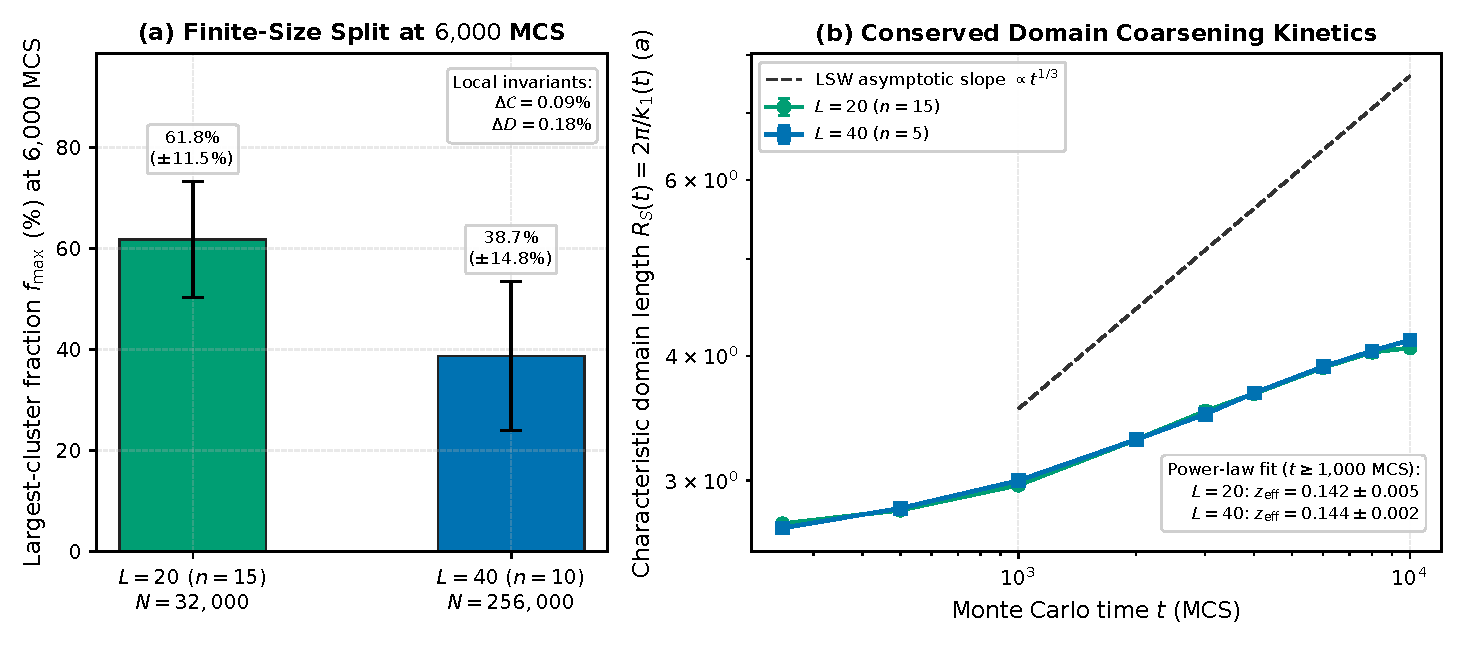
\includegraphics[width=0.96\textwidth]{fig08_finite_size_fcc.pdf}
  \caption{\label{fig:finite_size}Finite-size invariance and direct domain-coarsening kinetics for subcritical FCC ($C_v = 0.20, T = 2.00$). (a) At $6{,}000$ MCS, doubling system size from $L = 20$ ($n = 15$) to $L = 40$ ($n = 10$; error bars show $\pm 1\;\mathrm{SD}$) reduces $f_{\max}$ by $37.4\%$ while leaving local clustering $\mathcal{C}$ and diffusivity $D$ invariant to within $0.18\%$ (Table~\ref{tab:finite_size}). (b) Time-resolved structure-factor characteristic domain length $R_S(t) = 2\pi / k_1(t)$ ($L = 20$ $n = 15$, $L = 40$ $n = 5$; error bars show $\pm 1\;\mathrm{SE}$) collapses identically across both system sizes ($R_S(6{,}000) \approx 3.90\,a$) and grows with an effective preasymptotic exponent $z_{\mathrm{eff}} = 0.144 \pm 0.002$ ($t \ge 1{,}000$ MCS), substantially below the asymptotic $t^{1/3}$ LSW slope (dashed reference line)~\cite{Huse1986,Amar1988,Majumder2011}.}
\end{figure*}


Direct time-resolved measurement of the structure-factor characteristic length $R_S(t) = 2\pi / k_1(t)$ [Eq.~\eqref{eq:structure_factor_R}] up to $t = 10{,}000$ MCS provides direct evidence for the physical mechanism underlying this finite-size separation [Fig.~\ref{fig:finite_size}(b)]. Across the interval $t \in [250, 8{,}000]$ MCS, the measured $R_S(t)$ trajectories for $L = 20$ and $L = 40$ nearly superimpose, reaching $R_S(6{,}000) = 3.892 \pm 0.041\,a$ ($L = 20$) and $3.900 \pm 0.017\,a$ ($L = 40$), a relative difference of just $0.21\%$ ($p = 0.859$). Thus, physical domains reach approximately the same characteristic length, $R_S(6{,}000) \approx 3.90\,a$, in both systems. Doubling $L$ consequently halves the dimensionless ratio $R_S/L$ from $0.195$ to $0.098$. This change is consistent with the observed reduction in the fraction of vacancies incorporated into the largest connected component ($f_{\max}$), while local clustering ($\mathcal{C}$), diffusivity ($D$), and the measured characteristic domain length remain statistically consistent between the two sizes. Moreover, tracking $P_{\mathrm{span}}(t)$ along these trajectories reveals why subcritical FCC can initially span despite subsequently developing disconnected compact domains. At early times ($t \leq 1{,}000$ MCS), dispersed vacancies span all boxes ($P_{\mathrm{span}} = 1.00$, $f_{\max} = 74\%$--$80\%$). As the droplets compact, the trajectories show a progressive loss of system-spanning connections: $P_{\mathrm{span}}$ decreases to $0.40$--$0.47$ by $6{,}000$ MCS and $0.20$--$0.27$ by $10{,}000$ MCS.

Fitting $R_S(t) \propto t^{z_{\mathrm{eff}}}$ over $t \in [1{,}000, 10{,}000]$ MCS yields effective preasymptotic growth exponents of $z_{\mathrm{eff}} = 0.142 \pm 0.005$ (regression SE; $95\%$ CI $[0.132, 0.152]$, $R^2 = 0.993$) at $L = 20$ and $z_{\mathrm{eff}} = 0.144 \pm 0.002$ (regression SE, $R^2 = 0.999$) at $L = 40$. At $L = 40$, the exponent remains $0.145 \pm 0.004$ over $t \geq 2{,}000$ MCS, whereas at $L = 20$ it decreases slightly to $0.135 \pm 0.007$ as $R_S/L$ approaches $0.20$. The inverse interface-density measure exhibits a smaller apparent growth exponent, $z_{\mathrm{int}} = 0.075 \pm 0.002$ ($L = 40$), because thermally excited vacancies in the atom-rich matrix contribute a nonzero background to $\langle z_{\mathrm{av}}\rangle$. Importantly, $z_{\mathrm{eff}} \approx 0.144$ is substantially smaller than the classical asymptotic LSW value of $1/3$. Our trajectories, extending only to $10^4$ MCS, do not independently establish the asymptotic LSW exponent. Instead, the measured exponent characterizes the slow effective growth observed within the accessible preasymptotic conserved Kawasaki coarsening regime, where interfacial diffusion and curvature corrections can suppress early-to-intermediate growth rates below the asymptotic $1/3$ value \cite{Huse1986,Amar1988,Majumder2011}.

\begin{table*}[t]
\caption{\label{tab:finite_size}Expanded finite-size benchmark and direct coarsening kinetics for subcritical FCC ($C_v = 0.20$, $T = 2.00$). At $t = 6{,}000$ MCS, reported values are ensemble mean $\pm$ SD (with SE in parentheses) for $f_{\max}$, final $\mathcal{C}$, production-window $\bar{\mathcal{C}}$, diffusivity $D$, and structure-factor domain length $R_S$. Spanning probabilities are reported with $95\%$ Wilson confidence intervals. The effective preasymptotic growth exponent $z_{\mathrm{eff}}$ is fitted to $R_S(t)$ over $t \in [1{,}000, 10{,}000]$ MCS and is reported as the fitted estimate $\pm$ regression SE ($n = 15$ for $L = 20$; $n = 10$ up to $6{,}000$ MCS and $n = 5$ up to $10{,}000$ MCS for $L = 40$).}
\begingroup
\footnotesize
\setlength{\tabcolsep}{5pt}
\begin{ruledtabular}
\begin{tabular}{lccc}
Observable & $L = 20$ ($N = 32{,}000$, $n = 15$) & $L = 40$ ($N = 256{,}000$, $n = 10$) & Rel.\ diff.\ ($p_{\mathrm{Welch}}$) \\
\colrule
$f_{\max}$ (\%) at $6{,}000$ MCS & $61.8 \pm 11.5$ ($3.0$) & $38.7 \pm 14.8$ ($4.7$) & $-37.4\%$ ($7.1 \times 10^{-4}$) \\
$P_{\mathrm{span}}$ [$95\%$ Wilson CI] & $0.467$ [$0.248, 0.699$] & $0.400$ [$0.168, 0.687$] & --- \\
Final clustering $\mathcal{C}$ & $2.386 \pm 0.073$ ($0.019$) & $2.384 \pm 0.021$ ($0.007$) & $-0.09\%$ ($0.917$) \\
Window clustering $\bar{\mathcal{C}}$ & $2.294 \pm 0.048$ ($0.012$) & $2.283 \pm 0.014$ ($0.004$) & $-0.47\%$ ($0.421$) \\
Diffusivity $D$ ($10^{-2}\,a^2/\mathrm{MCS}$) & $1.204 \pm 0.017$ ($0.004$) & $1.206 \pm 0.007$ ($0.002$) & $+0.18\%$ ($0.660$) \\
Domain length $R_S(6{,}000)$ ($a$) & $3.892 \pm 0.160$ ($0.041$) & $3.900 \pm 0.053$ ($0.017$) & $+0.21\%$ ($0.859$) \\
Coarsening exponent $z_{\mathrm{eff}}$ ($t \geq 10^3$, fit $\pm$ SE) & $0.142 \pm 0.005$ & $0.144 \pm 0.002$ & --- \\
\end{tabular}
\end{ruledtabular}
\endgroup
\end{table*}

\subsection{Empirically Fitted Cross-Lattice Transport Scaling and Out-of-Sample Validation}
\label{sec:reduced_scaling}

Normalizing diffusivity by the analytical dilute-limit lattice scale $D_{\mathrm{ref}} = \frac{1}{3}f_0 r_{\mathrm{nn}}^2$ (Table~\ref{tab:lattice_specs}), concentration by $p_c$, and temperature by $T_c$ provides a useful framework for organizing transport across SC, BCC, and FCC. We first test whether diffusivity can be described using a single composite variable,

\begin{equation}
\Lambda = \left(\frac{C_v}{p_c}\right)\left(\frac{T_c}{T}\right).
\label{eq:lambda}
\end{equation}

As detailed in Appendix~\ref{app:diagnostics} (Fig.~\ref{fig:lambda_transport}), this single-variable description fails to capture the observed transport variation. Pooled regression of $\ln(D/D_{\mathrm{ref}})$ on $\ln\Lambda$ gives $R^2 = 0.068$ (slope $-0.194 \pm 0.033$; $R^2 = 0.024$ under $D/D_{\mathrm{scale}}$), with distinct negative per-lattice slopes of $-0.505 \pm 0.073$ (SC), $-0.328 \pm 0.098$ (BCC), and $-0.281 \pm 0.055$ (FCC).

Allowing $C_v/p_c$ and $T/T_c$ to enter independently through fitted exponents,

\begin{equation}
\ln\!\left(\frac{D}{D_{\mathrm{ref}}}\right)
=
a + \alpha \ln\!\left(\frac{C_v}{p_c}\right)
+ \beta \ln\!\left(\frac{T}{T_c}\right),
\label{eq:two_param_log}
\end{equation}

or equivalently,

\begin{equation}
\frac{D}{D_{\mathrm{ref}}}
=
A\left(\frac{C_v}{p_c}\right)^\alpha
\left(\frac{T}{T_c}\right)^\beta,
\qquad A=e^a,
\end{equation}

provides a substantially better description of all $465$ canonical trajectories [Fig.~\ref{fig:master_curve}(a) and Table~\ref{tab:scaling_fits}]. Although $D_{\mathrm{ref}}$ is an analytical dilute-limit normalization with no fitted parameters, the amplitude $A$ and exponents $(\alpha,\beta)$ are empirically fitted. Equation~\eqref{eq:two_param_log} should therefore be interpreted as an empirical two-variable scaling relationship built upon an analytical lattice normalization, rather than a parameter-free theoretical law. Pooled OLS yields

\begin{align}
a &= -2.1297 \pm 0.0044 \qquad (A = 0.1189), \nonumber \\
\alpha &= +0.6280 \pm 0.0131, \nonumber \\
\beta &= +1.0747 \pm 0.0136,
\label{eq:free_fit_params}
\end{align}

achieving $R^2_{\log} = 0.9407$, linear-space $R^2_{\mathrm{lin}} = 0.9381$, $\mathrm{RMSE}_{\log} = 0.0747$, and $\mathrm{MAPE} = 6.37\%$. The positive temperature exponent $\beta = +1.075 \pm 0.014$ captures the increase in diffusivity with temperature, while the sublinear concentration exponent $\alpha = 0.628 \pm 0.013$ lies within the individual within-lattice range $\alpha_g \in [0.580,0.703]$ (Table~\ref{tab:scaling_fits}).

Equation~\eqref{eq:two_param_log} also explains why the single-variable hypothesis based on $\Lambda$ fails. Substituting $\ln(C_v/p_c) = \ln\Lambda - \ln(T_c/T)$ gives

\begin{equation}
\ln\!\left(\frac{D}{D_{\mathrm{ref}}}\right)
=
a + \alpha\ln\Lambda
-(\alpha+\beta)\ln\!\left(\frac{T_c}{T}\right).
\label{eq:lambda_identity}
\end{equation}

Because both $\alpha$ and $\beta$ are positive, increasing concentration at fixed temperature raises $\ln(D/D_{\mathrm{ref}})$ with slope $+\alpha$ in a plot of $\ln(D/D_{\mathrm{ref}})$ against $\ln\Lambda$. Conversely, cooling at fixed concentration increases $\ln\Lambda$ while lowering $\ln(D/D_{\mathrm{ref}})$, giving a slope $-\beta$ along a fixed-concentration branch. Combining these distinct trends into a single predictor therefore mixes opposing concentration and temperature effects and produces misleading negative pooled slopes (Fig.~\ref{fig:lambda_transport}).

For comparison, Fig.~\ref{fig:master_curve}(b) and Table~\ref{tab:scaling_fits} also evaluate a constrained rational-exponent approximation,

\begin{equation}
\frac{D}{D_{\mathrm{ref}}}
=
0.1225
\left(\frac{C_v}{p_c}\right)^{3/4}
\left(\frac{T}{T_c}\right),
\label{eq:master_scaling}
\end{equation}

which fits only the amplitude $A$ while fixing the exponents at $(3/4,1)$. This approximation achieves $R^2_{\log} = 0.9222$ and $R^2_{\mathrm{lin}} = 0.9339$ ($\mathrm{MAPE} = 7.03\%$). The free-exponent model provides a better log-space fit, with $\Delta R^2_{\log} = +0.0185$, while the constrained expression remains a compact approximation. The fitted exponent $\alpha = 0.628 \pm 0.013$ is consistent with the sublinear concentration dependence observed individually across all three lattice topologies.

Grouped out-of-sample cross-validation further demonstrates that the empirical relationship retains predictive accuracy beyond the conditions used for fitting (Table~\ref{tab:scaling_fits}):

\begin{itemize}
\item \textbf{Leave-One-Condition-Out CV ($31$ folds):} Holding out all $15$ seeds belonging to each condition gives $R^2_{\mathrm{CV,log}} = 0.9252$ ($R^2_{\mathrm{CV,lin}} = 0.9205$, $\mathrm{MAPE} = 7.13\%$) for the free model and $0.9171$ ($R^2_{\mathrm{CV,lin}} = 0.9295$, $\mathrm{MAPE} = 7.26\%$) for the constrained $(3/4,+1)$ model.

\item \textbf{Stratified $5$-Fold Grouped Condition CV:} The free model achieves $R^2_{\mathrm{CV,log}} = 0.9320$ ($\mathrm{MAPE} = 6.84\%$), compared with $0.9193$ ($\mathrm{MAPE} = 7.22\%$) for the constrained model.

\item \textbf{Leave-One-Lattice-Out CV ($3$ folds):} Training on two lattice topologies and predicting the third without recalibration gives an overall $R^2_{\mathrm{CV,log}} = 0.9297$ ($R^2_{\mathrm{CV,lin}} = 0.9249$, $\mathrm{MAPE} = 6.78\%$) for the free model. The held-out lattice results are $R^2_{\log} = 0.9179$ for SC ($\mathrm{MAPE} = 8.90\%$), $0.9399$ for BCC ($6.13\%$), and $0.9354$ for FCC ($5.83\%$, $R^2_{\mathrm{lin}} = 0.9545$). The constrained model achieves an overall $R^2_{\mathrm{CV,log}} = 0.9080$.
\end{itemize}

\begin{figure*}[t]
  \centering
  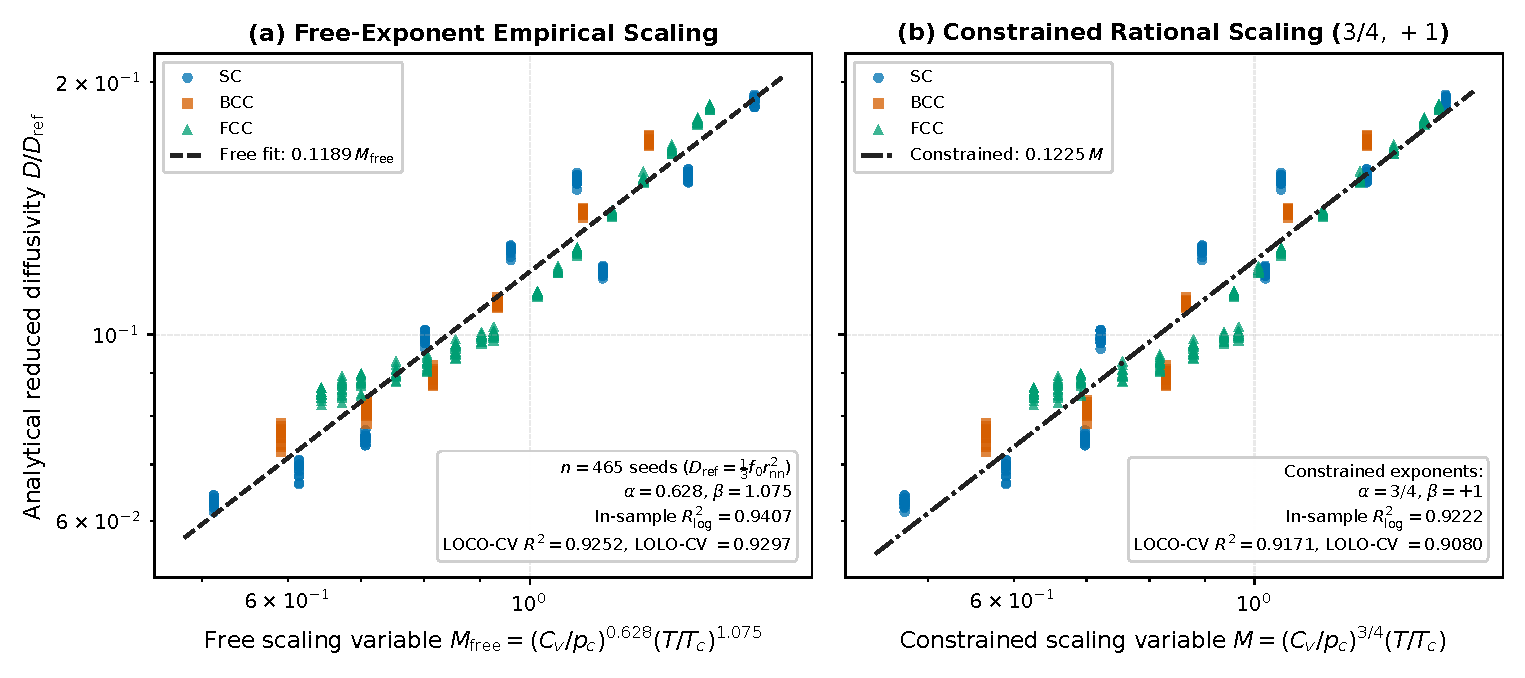
\includegraphics[width=0.96\textwidth]{fig09_two_param_master_curve.pdf}
  \caption{\label{fig:master_curve}Empirically fitted two-variable cross-lattice transport scaling of all $n=465$ canonical trajectories, normalized by the analytical dilute-limit diffusivity $D_{\mathrm{ref}}=\frac{1}{3}f_0r_{\mathrm{nn}}^2$. (a) Free-exponent fit, $D/D_{\mathrm{ref}}=0.1189(C_v/p_c)^{0.628}(T/T_c)^{1.075}$ ($R^2_{\log}=0.9407$, $31$-fold LOCO-CV $R^2_{\mathrm{CV,log}}=0.9252$, and $3$-fold Leave-One-Lattice-Out CV $R^2_{\mathrm{CV,log}}=0.9297$). (b) Constrained rational-exponent approximation, $D/D_{\mathrm{ref}}=0.1225(C_v/p_c)^{3/4}(T/T_c)$ ($R^2_{\log}=0.9222$, LOCO-CV $0.9171$, and LOLO-CV $0.9080$).}
\end{figure*}

Comparing $D/D_{\mathrm{ref}}$ with the secondary empirical normalization $D/D_{\mathrm{scale}}$ (Table~\ref{tab:scaling_fits}) further clarifies the importance of the analytical normalization. Because $p_c$ decreases from SC to FCC, the three lattices span staggered $C_v/p_c$ intervals. Under $D_{\mathrm{scale}}$, per-lattice fitted amplitudes drift from $A=0.1415$ to $0.1462$ to $0.1532$, introducing a topology-dependent offset that raises the pooled concentration exponent to $\alpha=0.742\pm0.015$, above every within-lattice estimate ($\alpha_g\in[0.580,0.703]$). This normalization also increases the lattice-specific contribution to $R^2_{\log}$ by $2.01$ percentage points ($F(6,456)=29.34$, $p=9.95\times10^{-30}$) and reduces Leave-One-Lattice-Out predictive performance to $R^2_{\mathrm{CV,log}}=0.8737$.

Under the analytical normalization $D_{\mathrm{ref}}$, per-lattice amplitudes align more closely ($A=0.1228$, $0.1196$, and $0.1183$ for SC, BCC, and FCC, respectively). The additional explanatory contribution of lattice-specific parameters is correspondingly smaller, with an increase of $0.43$ percentage points in $R^2_{\log}$ ($R^2_{\log,\mathrm{sep}}=0.9449$ versus pooled $R^2_{\log}=0.9407$). The nested $F$-test nevertheless detects statistically significant residual topology dependence ($F(6,456)=5.91$, $p=5.97\times10^{-6}$), indicating that the analytical normalization does not eliminate all lattice-specific transport effects.

Restricting the analysis to the strictly matched two-temperature subset ($n=420$, excluding SC $T/T_c=1.77$) preserves high predictive accuracy ($R^2_{\log}=0.9506$, LOCO-CV $R^2_{\mathrm{CV,log}}=0.9401$) while shifting the fitted exponents to $\alpha=0.575$ and $\beta=1.177$. This sensitivity further indicates that the fitted exponents are effective empirical parameters over the sampled regime rather than exact fundamental constants. By comparison, fitting $\ln f_{\max}$ using the same two reduced variables achieves only $R^2=0.6531$ ($\alpha=2.611$, $\beta=-1.517$), showing that the same scaling form is substantially less effective for predicting global cluster morphology.

\begin{table*}[t]
\caption{\label{tab:scaling_fits}Empirically fitted two-variable cross-lattice transport scaling, $\ln(D/D_{\mathrm{norm}}) = a + \alpha \ln(C_v/p_c) + \beta \ln(T/T_c)$, and grouped out-of-sample cross-validation ($31$-fold LOCO-CV, $5$-fold grouped CV, and $3$-fold Leave-One-Lattice-Out LOLO-CV) across all $n = 465$ canonical trajectories. Primary rows use the zero-free-parameter analytical normalization $D_{\mathrm{ref}} = \frac{1}{3}f_0 r_{\mathrm{nn}}^2$; bottom rows compare empirical $D_{\mathrm{scale}}$ and the matched two-temperature subset ($n = 420$, excluding SC $T/T_c = 1.77$). Nested shared-versus-lattice-specific model comparisons give $F(6,456)=5.91$ ($p=5.97\times10^{-6}$), corresponding to an increase of $0.43$ percentage points in $R^2_{\log}$ for $D/D_{\mathrm{ref}}$, and $F(6,456)=29.34$ ($p=9.95\times10^{-30}$), corresponding to an increase of $2.01$ percentage points for $D/D_{\mathrm{scale}}$.}
\begingroup
\footnotesize
\setlength{\tabcolsep}{3.5pt}
\begin{ruledtabular}
\begin{tabular}{lcccccccc}
Model / Subset & $n$ & $A = e^a$ & $\alpha$ ($C_v/p_c$) & $\beta$ ($T/T_c$) & $R^2_{\log}$ ($R^2_{\mathrm{lin}}$) & LOCO-CV & $5$-fold CV & LOLO-CV \\
\colrule
Primary $D/D_{\mathrm{ref}}$ (free) & $465$ & $0.1189$ & $0.628 \pm 0.013$ & $+1.075 \pm 0.014$ & $0.9407$ ($0.9381$) & $0.9252$ & $0.9320$ & $0.9297$ \\
Primary $D/D_{\mathrm{ref}}$ (constrained) & $465$ & $0.1225$ & $3/4$ & $+1$ & $0.9222$ ($0.9339$) & $0.9171$ & $0.9193$ & $0.9080$ \\
\colrule
SC $D/D_{\mathrm{ref}}$ (free)  & $135$ & $0.1228$ & $0.703 \pm 0.039$ & $+1.044 \pm 0.026$ & $0.9373$ & --- & --- & $0.9179$\footnotemark[1] \\
BCC $D/D_{\mathrm{ref}}$ (free) & $90$  & $0.1196$ & $0.590 \pm 0.031$ & $+1.214 \pm 0.030$ & $0.9580$ & --- & --- & $0.9399$\footnotemark[1] \\
FCC $D/D_{\mathrm{ref}}$ (free) & $240$ & $0.1183$ & $0.580 \pm 0.020$ & $+1.079 \pm 0.019$ & $0.9454$ & --- & --- & $0.9354$\footnotemark[1] \\
\colrule
Matched-$T$ $D/D_{\mathrm{ref}}$ (free) & $420$ & $0.1186$ & $0.575 \pm 0.012$ & $+1.177 \pm 0.015$ & $0.9506$ ($0.9505$) & $0.9401$ & --- & --- \\
Empirical $D/D_{\mathrm{scale}}$ (free) & $465$ & $0.1510$ & $0.742 \pm 0.015$ & $+1.040 \pm 0.015$ & $0.9279$ ($0.9379$) & $0.9092$ & $0.9205$ & $0.8737$ \\
Empirical $D/D_{\mathrm{scale}}$ (constrained) & $465$ & $0.1516$ & $3/4$ & $+1$ & $0.9266$ ($0.9381$) & $0.9218$ & $0.9237$ & $0.9150$ \\
\end{tabular}
\end{ruledtabular}
\footnotetext[1]{Per-lattice LOLO-CV $R^2_{\log}$ when that entire lattice is held out and predicted zero-shot from the other two lattices using the free $D/D_{\mathrm{ref}}$ fit.}
\endgroup
\end{table*}


\section{Discussion}
\label{sec:discussion}

\subsection{The Thermodynamic-to-Geometric Crossover and 3D Correlated Percolation}
\label{sec:crossover_discussion}

Our dilute benchmarks, $J=0$ random-occupancy controls, high-precision $n=50$ finite-time crossover measurements, matched-temperature comparisons, and three-dimensional morphological analyses reveal that thermodynamics and lattice geometry do not simply reinforce one another across $(T,C_v,Z)$ space.

In the dilute limit ($C_v\ll p_c$), vacancies diffuse nearly independently, with $D/C_v$ agreeing with the analytical dilute-limit reference $D_{\mathrm{ref}}=\frac{1}{3}f_0r_{\mathrm{nn}}^2$ within $+0.4\%$--$+0.8\%$ at $C_v=0.015$ and $+1.1\%$--$+1.9\%$ at $C_v=0.030$ (Table~\ref{tab:dilute_validation}). The small positive deviations are consistent with the weak finite-concentration correlation enhancement anticipated by lattice-gas kinetic theory \cite{Murch1977,Kehr1984}.

At intermediate concentrations below random site percolation ($C_v<p_c$, $T<T_{\mathrm{coex}}$), attractive interactions drive phase separation within the Ising miscibility gap, aggregating vacancies into compact domains and advancing finite-time spanning substantially below the corresponding $J=0$ crossover concentrations. This occurs in SC ($C_v^*/C_v^{*,J=0}=0.689$) and BCC ($C_v^*/C_v^{*,J=0}=0.881$). For BCC, the corresponding ratio to the infinite-lattice threshold is $C_v^*/p_c^{\mathrm{BCC}}=0.886$; these are different normalizations and should not be conflated. Heating above $T_c$ suppresses these domains, as reflected by the reduction in $f_{\max}$ in SC at $C_v=0.20$ and FCC at $C_v=0.15$, and by the decrease in BCC $f_{\max}$ from $63.6\%$ to $40.8\%$, although partial correlated connectivity remains near $p_c^{\mathrm{BCC}}$.

Near the geometric percolation scale ($C_v\gtrsim p_c(Z)$), attractive interactions influence connectivity in opposite directions below and above $T_c$. The direct $J=0$ versus $J=1$ comparison at FCC $C_v=0.20$ illustrates this competition (Table~\ref{tab:thermo_controls} and Fig.~\ref{fig:fcc_3way}). Uncorrelated random occupancy ($J=0$, $\mathcal{C}=1.00$) places FCC close to its random percolation threshold, with $f_{\max}=33.3\%$ and $P_{\mathrm{span}}=0.480$. Above $T_c$ ($T/T_c=1.25$), the FCC lattice provides a highly connected geometric framework, while residual short-range attractive correlations ($\mathcal{C}=1.30$) shift the spanning crossover downward to $C_v^*=0.1761$, approximately $0.882\,p_c^{\mathrm{FCC}}$ using $p_c^{\mathrm{FCC}}=0.1996$. At $C_v=0.20$, this produces a space-filling spanning network ($f_{\max}=73.9\%$, $P_{\mathrm{span}}=1.00$). Below $T_c$, however, strong attractive interactions compact vacancies into dense coarsening droplets ($\mathcal{C}=2.38$), delaying finite-time spanning slightly beyond the random geometric reference ($C_v^*=0.2083=1.044\,p_c^{\mathrm{FCC}}$, $95\%$ CI $[1.024,1.065]$). Thus, the same attractive interaction can advance spanning above $T_c$ while delaying it below $T_c$, depending on whether short-range correlations promote connected occupancy or phase separation produces compact, disconnected droplets.

These findings complement equilibrium studies of three-dimensional correlated Ising percolation while highlighting the distinct role of conserved dynamics and finite coarsening time. Classical Monte Carlo investigations by Müller-Krumbhaar \cite{MullerKrumbhaar1974}, Coniglio and Klein \cite{Coniglio1980}, Kertész \cite{Kertesz1989}, and D'Onorio de Meo, Heermann, and Binder \cite{DOnorioDeMeo1990} examined how attractive spin couplings shift geometric-cluster percolation away from random $p_c$ and define the supercritical Kertész line. Two-dimensional analyses further clarified the relationship between geometric spin clusters and thermal criticality \cite{Fortunato2002}. More recently, equilibrium simulations by Zhu \textit{et al.} \cite{Zhu2026} established a single percolation transition for geometric spin clusters in the critical three-dimensional Ising model, contrasting with the consecutive transitions reported in two dimensions.

Our supercritical FCC crossover shift is qualitatively consistent with the enhanced connectivity associated with attractive correlations in three-dimensional equilibrium systems. Above $T_c$, the detailed-balance dynamics has the canonical fixed-magnetization distribution as its stationary distribution; residual short-range correlations in the finite-time configurations can therefore influence geometric connectivity. Below $T_c$, however, our investigation addresses a different physical regime: conserved-magnetization Kawasaki dynamics inside the miscibility gap at finite coarsening age. We analyze pure nearest-neighbor geometric vacancy clusters rather than Coniglio--Klein bonded physical droplets \cite{Coniglio1980,DOnorioDeMeo1990} or equilibrium critical spin configurations \cite{Zhu2026}. In this regime, aggregation can either advance or delay periodic spanning depending on whether growing domains bridge sparse lattice networks, as observed in SC and BCC, or compact into disconnected droplets, as observed in FCC.

\subsection{Why Time-Aligned Local Coordination Outperforms Global Connectivity}
\label{sec:morphology_vs_transport}

The relationship between $f_{\max}$ and transport depends on whether differences are assessed across conditions or among seeds within the same condition. In the pooled covariate-controlled regression, $f_{\max}$ has a positive coefficient, whereas its bivariate association with diffusivity is weak and its within-lattice correlations have opposite signs across topologies (Table~\ref{tab:struct_transport}). These pooled results describe between-condition contrasts and should not be interpreted as evidence that larger clusters increase diffusivity within a fixed condition. Once condition-specific intercepts are included, the within-condition association is negligible ($R^2_{\mathrm{within}}=0.0044$, $p_{\mathrm{WCB}}=0.309$). This distinction is physically reasonable: atomic mobility depends on local vacancy availability and the energy barriers associated with individual exchange events, not simply on whether distant vacancies belong to the same periodically connected cluster.

The expanded $L=20$ to $L=40$ benchmark, together with direct $R_S(t)$ measurements (Fig.~\ref{fig:finite_size}), demonstrates this separation quantitatively. At $6{,}000$ MCS, the physical characteristic domain length remains approximately $3.90\,a$ in both systems. Doubling the box size therefore reduces $R_S/L$ and lowers $f_{\max}$ by $37.4\%$, while production-window clustering and diffusivity remain consistent within $0.47\%$ and $0.18\%$, respectively. The measured effective growth exponent $z_{\mathrm{eff}}=0.144\pm0.002$ characterizes the preasymptotic coarsening regime accessible to these simulations; it does not establish the asymptotic $t^{1/3}$ LSW limit.

By contrast, local vacancy coordination is directly related to the atom--vacancy interface density and exchange attempt frequency $\Gamma_{\mathrm{att}}$. Exact bond conservation [Eq.~\eqref{eq:bond_conservation}] links increased local vacancy clustering $\mathcal{C}$ to a reduction in the number of atom--vacancy interfacial bonds, providing a microscopic basis for the observed conditional association between clustering and diffusivity.

Our condition-fixed-effects analysis further shows that this association persists when concentration, temperature, and lattice topology are held fixed, particularly in the subcritical ensemble. Across all $31$ conditions, production-window clustering $\bar{\mathcal{C}}$ accounts for $49.5\%$ of within-condition seed-to-seed $\ln D$ variance, increasing to $68.0\%$ across the $14$ subcritical conditions ($p_{\mathrm{WCB}}\leq0.0003$). This exceeds the corresponding explanatory contribution of final-snapshot clustering $\mathcal{C}$ ($20.8\%$). The stronger association for production-window measurements is consistent with the fact that diffusivity accumulates over a trajectory, whereas a final snapshot captures only one instant.

Nevertheless, this conditional association does not establish that $\bar{\mathcal{C}}$ alone causally determines diffusivity. Distinct controlled slopes across topologies ($-1.287$ for SC, $-1.029$ for BCC, and $-0.939$ for FCC) indicate that coordination-dependent activation spectra, with $\Delta E\in[-ZJ,+ZJ]$, and tracer correlation factors $f(C_v,T,Z)$ also contribute to atomic mobility \cite{Kehr1984,Kehr1989}.

\subsection{Interpretation and Generalization of the Empirical Cross-Lattice Scaling Law}
\label{sec:scaling_interpretation}

Combining the analytical dilute-limit normalization $D_{\mathrm{ref}}=\frac{1}{3}f_0r_{\mathrm{nn}}^2$ with empirically fitted exponents on $C_v/p_c$ and $T/T_c$ captures $94.1\%$ of the pooled log-variance across the three studied cubic lattice topologies ($R^2_{\log}=0.9407$, MAPE $=6.37\%$). By comparison, the single-variable predictor $\Lambda=(C_v/p_c)(T_c/T)$ explains only $6.8\%$ of the pooled log-variance ($R^2=0.068$).

Over the sampled concentration interval $C_v\in[0.14,0.25]$, increasing vacancy concentration raises diffusivity, but attractive aggregation increasingly sequesters vacancies within clustered regions, reducing the effective concentration exponent below its dilute-limit value of unity. The resulting pooled exponent $\alpha=0.628\pm0.013$ lies within the range of individual lattice estimates ($\alpha_g\in[0.580,0.703]$). Simultaneously, across the sampled temperature interval $T/T_c\in[0.82,1.77]$, increasing temperature enhances diffusivity through higher exchange acceptance and thermal disruption of vacancy clusters. This behavior is captured by the fitted exponent $\beta=1.075\pm0.014$.

Grouped cross-validation demonstrates that the fitted relationship retains predictive accuracy when entire simulation conditions are excluded from training. Holding out all $15$ seeds belonging to each of the $31$ conditions gives LOCO-CV $R^2_{\mathrm{CV,log}}=0.9252$ and MAPE $=7.13\%$. More stringently, Leave-One-Lattice-Out validation gives an overall $R^2_{\mathrm{CV,log}}=0.9297$ and MAPE $=6.78\%$, when one of the three studied lattice topologies is withheld entirely during fitting.

This latter result demonstrates that the fitted relationship predicts transport across the three investigated cubic topologies without recalibrating its parameters for the held-out topology. It does not establish generalization to arbitrary crystal structures or lattice classes that were not included in the simulations.

Two qualifications remain important. First, the amplitude $A$ and exponents $(\alpha,\beta)$ are empirically fitted over the sampled parameter window rather than derived as exact theoretical constants. Their shift to $\alpha=0.575$ and $\beta=1.177$ in the restricted matched-temperature subset ($n=420$) illustrates their sensitivity to the sampled temperature range. Second, the nested $F$-test ($F(6,456)=5.91$, $p=5.97\times10^{-6}$) detects statistically significant residual topology dependence, despite the relatively small improvement of $0.43$ percentage points in $R^2_{\log}$. The fitted relationship therefore provides an approximate empirical scaling law across the three investigated cubic lattices and over the sampled parameter regime, rather than an exact universal description of vacancy transport.

\subsection{Model Scope and Future Directions}
\label{sec:limitations}

Four natural extensions define the scope of the present results.

First, our lattice-gas Hamiltonian includes only isotropic nearest-neighbor attractions. Real crystalline materials introduce additional effects, including elastic strain fields, longer-range defect interactions, and configuration-dependent saddle-point migration barriers, which are not represented by the present Metropolis Kawasaki model.

Second, although $L=40$ establishes finite-size consistency of $D$, $\mathcal{C}$, and $R_S(t)$ over the investigated subcritical FCC conditions, it does not establish complete finite-size convergence of every morphological observable. Extending interacting coarsening simulations to $t\geq10^5$ MCS across $L\in\{20,40,60\}$ would allow the evolution of the measured preasymptotic growth regime to be followed over a substantially longer timescale and would help determine whether the effective exponent approaches the asymptotic LSW value of $1/3$ \cite{Huse1986,Majumder2011}. The existing $L\in\{20,30,40\}$ random-percolation controls provide a separate finite-size benchmark for the non-interacting system.

Third, wider temperature and concentration intervals are needed to establish the validity boundaries of the empirical scaling law. At low temperatures, activated transport and Arrhenius behavior may become dominant, whereas at high temperatures, saturation of Metropolis exchange acceptance may introduce curvature that cannot be captured by a simple power law. Lower concentrations, approaching the dilute limit where the concentration exponent tends toward unity, and additional crystal structures, such as HCP and diamond cubic, would provide important tests of the proposed scaling relationship.

Finally, mapping the finite-time spanning crossover throughout the $(T/T_c,C_v/p_c)$ plane would help distinguish thermodynamic aggregation from geometric percolation more systematically. Comparing these crossover curves with transport iso-contours would provide a broader framework for understanding the relationship between equilibrium correlated percolation, conserved vacancy coarsening, and kinetic vacancy diffusion \cite{Kertesz1989,DOnorioDeMeo1990,Zhu2026}.


\section{Conclusions}
\label{sec:conclusions}

By comparing SC, BCC, and FCC lattices across $1{,}740$ unique interacting conserved Kawasaki Monte Carlo trajectories, comprising $465$ canonical runs, $n=50$-seed finite-time percolation crossover sweeps, $90$ high-temperature dilute validations, and expanded $L=40$ coarsening runs, together with $8{,}200$ non-interacting $J=0$ random-percolation controls, we establish four principal findings.

First, thermodynamics and lattice geometry influence vacancy connectivity in competing ways. In the dilute limit, all three lattices recover the analytical dilute-limit transport normalization $D_{\mathrm{ref}}=\frac{1}{3}f_0r_{\mathrm{nn}}^2$ within $+0.4\%$--$+0.8\%$ at $C_v=0.015$ and $+1.1\%$--$+1.9\%$ at $C_v=0.030$. At matched subcritical temperatures ($T/T_c\simeq0.82$), attractive aggregation advances finite-time spanning crossovers below the corresponding random-occupancy references in SC ($C_v^*/C_v^{*,J=0}=0.689$) and BCC ($C_v^*/C_v^{*,J=0}=0.881$; equivalently, $C_v^*/p_c^{\mathrm{BCC}}=0.886$). In FCC, however, compact droplet formation slightly delays the finite-time spanning crossover beyond its random reference ($1.044\,p_c^{\mathrm{FCC}}$, $95\%$ CI $[1.024,1.065]$). For BCC, the crossover is $0.886$ times the infinite-lattice threshold and $0.881$ times the measured finite-size $J=0$ crossover. Above $T_c$, residual attractive correlations instead shift the FCC crossover downward ($0.882\,p_c^{\mathrm{FCC}}$), producing a space-filling spanning network at $C_v=0.20$. These results demonstrate that attractive interactions do not universally enhance global vacancy connectivity: their effect depends on temperature, lattice geometry, and the evolving morphology of vacancy aggregates.

Second, local vacancy coordination is more informative about atomic transport than global cluster connectivity within fixed simulation conditions. Under condition-fixed-effects regression, production-window clustering $\bar{\mathcal{C}}$ accounts for $49.5\%$ of within-condition seed-to-seed $\ln D$ variance across all $31$ conditions, increasing to $68.0\%$ across the $14$ subcritical conditions ($p_{\mathrm{WCB}}=0.0003$). In contrast, $f_{\max}$ shows negligible within-condition explanatory power ($R^2_{\mathrm{within}}=0.0044$, $p_{\mathrm{WCB}}=0.309$). These findings support the importance of local exchange environments for transport, while showing that global cluster size alone is insufficient to predict tracer mobility. The observed clustering--diffusivity relationship is conditional and does not establish that clustering alone causally determines diffusion.

Third, macroscopic connectivity exhibits a stronger finite-size dependence than local transport in the investigated subcritical FCC benchmark. Increasing the system size from $L=20$ to $L=40$ reduces $f_{\max}$ by $37.4\%$, while the characteristic physical domain length remains approximately $3.90\,a$ at $6{,}000$ MCS. Local clustering and diffusivity remain consistent within $0.47\%$ and $0.18\%$, respectively. The measured effective coarsening exponent $z_{\mathrm{eff}}=0.144\pm0.002$ characterizes the preasymptotic growth regime accessible to our simulations; longer trajectories are required to establish the subsequent approach, if any, toward asymptotic LSW growth.

Fourth, tracer diffusivity across the three studied cubic lattice topologies follows the empirically fitted two-variable scaling relationship

\begin{equation}
\frac{D}{D_{\mathrm{ref}}}
=
0.1189
\left(\frac{C_v}{p_c}\right)^{0.628}
\left(\frac{T}{T_c}\right)^{1.075},
\end{equation}

with $R^2_{\log}=0.9407$ and MAPE $=6.37\%$. The relationship retains predictive accuracy under Leave-One-Condition-Out validation ($R^2_{\mathrm{CV,log}}=0.9252$) and Leave-One-Lattice-Out validation ($R^2_{\mathrm{CV,log}}=0.9297$), demonstrating predictive transfer among the three studied cubic topologies, SC, BCC, and FCC, without recalibration for the held-out topology. Nevertheless, statistically significant residual topology dependence remains, with lattice-specific parameters improving $R^2_{\log}$ by $0.43$ percentage points. The fitted relationship should therefore be interpreted as an approximate empirical scaling law over the investigated parameter range rather than an exact universal law.

Together, these results establish that vacancy transport, spatial aggregation, and global percolation are related but distinct phenomena. Local atomic exchange environments are more informative about transport than macroscopic connectivity, while the competition between thermodynamic aggregation and lattice geometry determines whether vacancy clusters advance or suppress finite-time spanning.

\section*{Data and Code Availability}

The Numba-accelerated Kawasaki Monte Carlo engine, periodic wrapping analyzer, three-dimensional structure-factor coarsening diagnostics, automated $22$-test verification suite (\texttt{pytest}), statistical and condition-fixed-effects pipelines, cross-validation scripts, figure-generation scripts, raw datasets, and machine-readable summary statistics are available in the public
\href{https://github.com/salinode/lattice-vacancy-crossover}{GitHub repository}.

The repository contains the following data files:

\begingroup
\small
\ttfamily
\raggedright
\setlength{\parskip}{1.5pt}
\path{seed_level_465.csv}\par
\path{dilute_validation.csv}\par
\path{random_percolation_j0.csv}\par
\path{percolation_high_precision.csv}\par
\path{spanning_dense_subcritical.csv}\par
\path{fcc_concentration_sweep.csv}\par
\path{thermo_controls.csv}\par
\path{finite_size_fcc.csv}\par
\path{coarsening_kinetics.csv}\par
\path{summary_stats.json}
\endgroup

The repository also provides the input parameters, deterministic seed-generation procedure, raw trajectory-level data, and analysis scripts needed to reproduce the reported results. Every reported trajectory, bootstrap interval, and fixed-effects statistic is intended to be reproducible using the documented deterministic SHA-256 seed schedule.

\appendix

\section{Single-Parameter Scaling Diagnostics and FCC Sweep Data}
\label{app:diagnostics}

Figures~\ref{fig:lambda_transport} and~\ref{fig:lambda_fmax} document the performance of the single-parameter description based on $\Lambda=(C_v/p_c)(T_c/T)$ for analytical reduced diffusivity $D/D_{\mathrm{ref}}$ and macroscopic cluster morphology $f_{\max}$ across all $n=465$ canonical trajectories.

\begin{center}
\begin{minipage}{\columnwidth}
\centering
\refstepcounter{figure}\label{fig:lambda_transport}
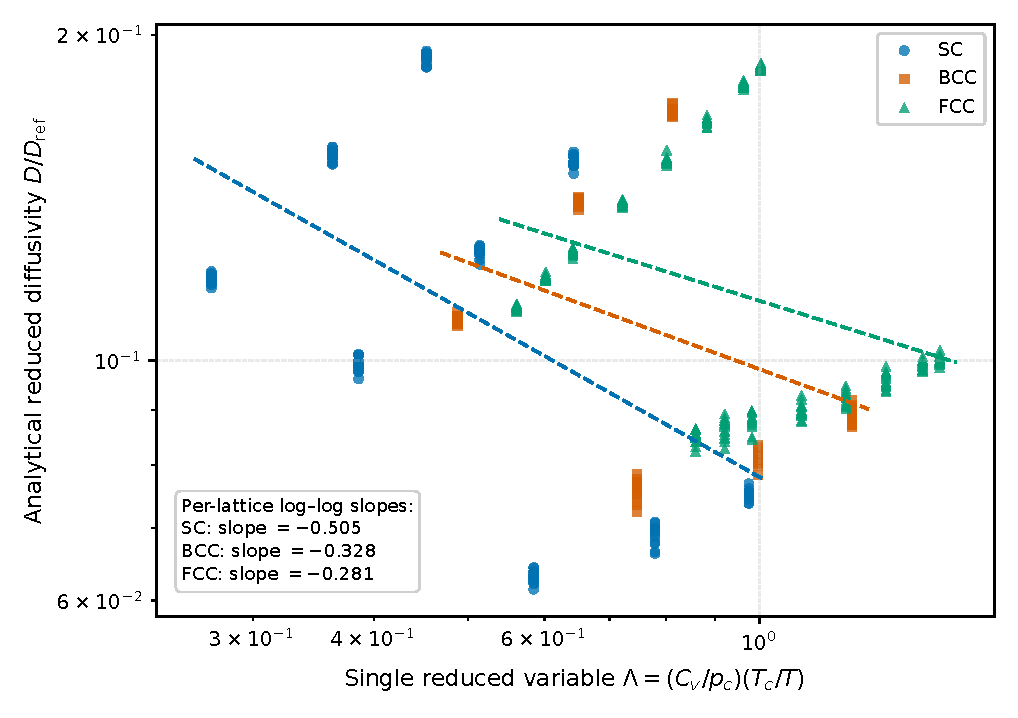
\includegraphics[width=\linewidth]{fig10_single_param_lambda_transport.pdf}
\par\smallskip
\raggedright\footnotesize\textbf{FIG. \thefigure.} Analytical reduced diffusivity $D/D_{\mathrm{ref}}$ versus the single composite variable $\Lambda=(C_v/p_c)(T_c/T)$ across all $n=465$ trajectories. Dashed lines show per-lattice log--log fits with distinct negative slopes ($-0.505$ for SC, $-0.328$ for BCC, and $-0.281$ for FCC; pooled $R^2=0.068$). Within each isotherm, $D/D_{\mathrm{ref}}$ increases with concentration and therefore with $\Lambda$, whereas cooling shifts the isothermal branches downward and toward larger $\Lambda$, illustrating the opposing contributions identified in Eq.~\eqref{eq:lambda_identity}.
\end{minipage}
\end{center}

In Fig.~\ref{fig:lambda_transport}, the opposing concentration and temperature trends appear as rising isothermal branches displaced downward and toward larger $\Lambda$ as temperature decreases. Regressing $\ln(D/D_{\mathrm{ref}})$ onto $\ln\Lambda$ alone yields weak, topology-dependent negative slopes: $-0.505\pm0.073$ ($R^2=0.264$) for SC, $-0.328\pm0.098$ ($R^2=0.112$) for BCC, $-0.281\pm0.055$ ($R^2=0.097$) for FCC, and $-0.194\pm0.033$ ($R^2=0.068$) for the pooled dataset (or $-0.118\pm0.035$, $R^2=0.024$ under $D/D_{\mathrm{scale}}$).

\begin{center}
\begin{minipage}{\columnwidth}
\centering
\refstepcounter{figure}\label{fig:lambda_fmax}
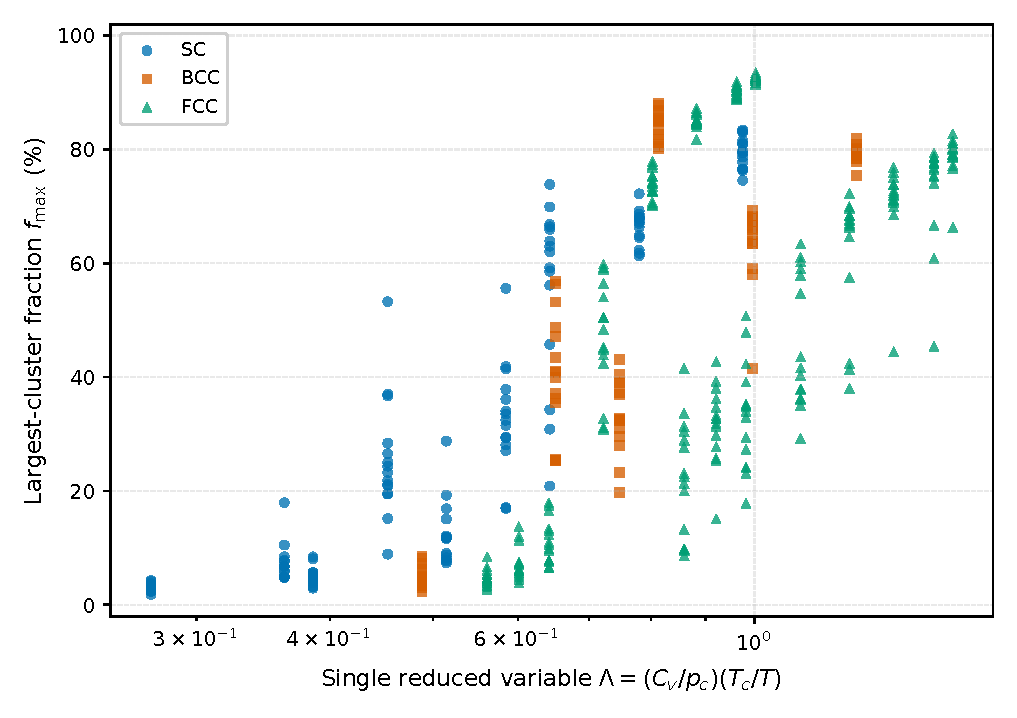
\includegraphics[width=\linewidth]{fig11_single_param_lambda_fmax.pdf}
\par\smallskip
\raggedright\footnotesize\textbf{FIG. \thefigure.} Largest-cluster fraction $f_{\max}$ versus $\Lambda=(C_v/p_c)(T_c/T)$ across all $n=465$ observations. The wide vertical spread at fixed $\Lambda$ indicates that finite-time morphology retains substantial dependence on lattice topology and coarsening history.
\end{minipage}
\end{center}

Figure~\ref{fig:lambda_fmax} shows $f_{\max}$ versus $\Lambda$. Although $f_{\max}$ increases broadly with $\Lambda$, the lattice branches span approximately $18\%$ to $93\%$ near $\Lambda\approx1.0$. Even the two-variable regression on $\ln(C_v/p_c)$ and $\ln(T/T_c)$ achieves only $R^2=0.6531$, indicating that these two reduced variables do not adequately capture the dependence of global cluster morphology on the simulation conditions.

Finally, Table~\ref{tab:fcc_sweep_full} compiles the complete canonical $15$-seed FCC concentration-sweep ensemble across all $16$ concentration-sweep conditions ($240$ trajectories), supporting Fig.~\ref{fig:fcc_sweep}.

% Set the final appendix table directly in the document flow so that the bibliography follows it without a deferred float page.
\onecolumngrid
\refstepcounter{table}
\label{tab:fcc_sweep_full}
\noindent\textbf{TABLE \thetable.} Canonical FCC concentration sweeps ($L=20$, $N=32{,}000$, $6{,}000$ MCS; $n=15$ seeds per condition) at $T=2.00$ ($T/T_c=0.816$) and $T=3.06$ ($T/T_c=1.249$). Entries are ensemble means $\pm$ SD for $f_{\max}$, $P_{\mathrm{span}}$, and $\mathcal{C}$, and means $\pm$ SE for $D$ in units of $10^{-2}\,a^2/\mathrm{MCS}$. The separate high-precision $n=50$ spanning-crossing analysis is reported in Table~\ref{tab:spanning}.
\par\vspace{5pt}
\begingroup
\small
\renewcommand{\arraystretch}{1.08}
\setlength{\tabcolsep}{7pt}
\begin{ruledtabular}
\begin{tabular*}{\textwidth}{@{\extracolsep{\fill}}cccccc}
\multicolumn{6}{l}{\textbf{(a) Below $T_c$: $T=2.00$, $T/T_c=0.816$}} \\
\colrule
$C_v$ & $C_v/p_c^{\mathrm{FCC}}$ & $f_{\max}$ (\%) & $P_{\mathrm{span}}$ & $\mathcal{C}$ & $D$ \\
\colrule
$0.14$ & $0.701$ & $22.1 \pm 10.3$ & $0.067$ & $1.91$ & $1.108 \pm 0.004$ \\
$0.15$ & $0.752$ & $31.7 \pm 6.7$ & $0.067$ & $2.15$ & $1.126 \pm 0.006$ \\
$0.16$ & $0.802$ & $33.2 \pm 9.3$ & $0.067$ & $2.24$ & $1.147 \pm 0.006$ \\
$0.18$ & $0.902$ & $46.3 \pm 11.7$ & $0.133$ & $2.38$ & $1.171 \pm 0.005$ \\
$0.20$ & $1.002$ & $61.8 \pm 11.5$ & $0.467$ & $2.39$ & $1.204 \pm 0.005$ \\
$0.22$ & $1.102$ & $70.7 \pm 7.6$ & $0.800$ & $2.36$ & $1.249 \pm 0.005$ \\
$0.24$ & $1.202$ & $73.2 \pm 9.2$ & $0.933$ & $2.31$ & $1.293 \pm 0.003$ \\
$0.25$ & $1.253$ & $78.8 \pm 3.8$ & $0.933$ & $2.25$ & $1.304 \pm 0.003$ \\
\colrule
\multicolumn{6}{l}{\textbf{(b) Above $T_c$: $T=3.06$, $T/T_c=1.249$}} \\
\colrule
$C_v$ & $C_v/p_c^{\mathrm{FCC}}$ & $f_{\max}$ (\%) & $P_{\mathrm{span}}$ & $\mathcal{C}$ & $D$ \\
\colrule
$0.14$ & $0.701$ & $4.7 \pm 1.5$ & $0.000$ & $1.33$ & $1.458 \pm 0.002$ \\
$0.15$ & $0.752$ & $7.1 \pm 2.9$ & $0.000$ & $1.32$ & $1.554 \pm 0.002$ \\
$0.16$ & $0.802$ & $11.2 \pm 3.8$ & $0.000$ & $1.32$ & $1.641 \pm 0.003$ \\
$0.18$ & $0.902$ & $47.3 \pm 9.9$ & $0.800$ & $1.32$ & $1.820 \pm 0.002$ \\
$0.20$ & $1.002$ & $73.9 \pm 2.4$ & $1.000$ & $1.30$ & $1.995 \pm 0.004$ \\
$0.22$ & $1.102$ & $85.1 \pm 1.3$ & $1.000$ & $1.30$ & $2.167 \pm 0.004$ \\
$0.24$ & $1.202$ & $90.2 \pm 1.0$ & $1.000$ & $1.29$ & $2.341 \pm 0.003$ \\
$0.25$ & $1.253$ & $92.5 \pm 0.5$ & $1.000$ & $1.28$ & $2.434 \pm 0.003$ \\
\end{tabular*}
\end{ruledtabular}
\endgroup
\twocolumngrid

\setlength{\bibsep}{0pt plus 0.25ex}
\bibliography{references}

\end{document}